%%%%%%%%%%%%%%%%%%%%%%%%%%%%%%%%%%%%%%%%%
% Mediolanum Internship Study Guide
% Built with the included Legrand Orange Book template
%%%%%%%%%%%%%%%%%%%%%%%%%%%%%%%%%%%%%%%%%

\documentclass[
	11pt,
	fleqn,
	a4paper,
	oneside,
]{LegrandOrangeBook}

\hypersetup{
	pdftitle={One-Week Study Guide for Banca Mediolanum Marketing Clienti Internship},
	pdfauthor={Prepared for a Computer Engineering Student},
	pdfsubject={Banking, CRM, Client Marketing, Segmentation, Marketing Automation, and ML},
	pdfkeywords={Banca Mediolanum, Marketing Clienti, CRM, Machine Learning, Segmentation, Banking},
	pdfcreator={LaTeX},
}

\addbibresource{sample.bib}

\definecolor{ocre}{RGB}{0, 92, 145}
\definecolor{medgreen}{RGB}{45, 139, 86}
\definecolor{medgray}{RGB}{77, 82, 88}
\definecolor{medamber}{RGB}{221, 143, 45}
\definecolor{medred}{RGB}{178, 64, 72}

\usepackage{tabularx}
\usepackage{longtable}
\usepackage{multicol}
\usepackage{ragged2e}
\usepackage{xurl}
\usepackage{pdflscape}
\usetikzlibrary{arrows.meta, positioning, shapes.geometric, calc, fit}

\chapterimage{header_study.jpg}
\chapterspaceabove{6.7cm}
\chapterspacebelow{7.3cm}

\setlength{\parindent}{0pt}
\setlength{\parskip}{5pt}
\renewcommand{\arraystretch}{1.18}
\newcolumntype{Y}{>{\RaggedRight\arraybackslash}X}

\tikzset{
	flow/.style={rectangle, rounded corners=4pt, draw=ocre!85, fill=ocre!8, line width=0.8pt, align=center, text width=3.0cm, minimum height=0.9cm, font=\sffamily\small},
	smallflow/.style={rectangle, rounded corners=3pt, draw=ocre!75, fill=ocre!7, line width=0.7pt, align=center, text width=2.3cm, minimum height=0.75cm, font=\sffamily\footnotesize},
	wideflow/.style={rectangle, rounded corners=4pt, draw=ocre!85, fill=ocre!8, line width=0.8pt, align=center, text width=4.1cm, minimum height=0.9cm, font=\sffamily\small},
	action/.style={rectangle, rounded corners=4pt, draw=medgreen!80!black, fill=medgreen!10, line width=0.8pt, align=center, text width=3.0cm, minimum height=0.9cm, font=\sffamily\small},
	risk/.style={rectangle, rounded corners=4pt, draw=medred!85, fill=medred!8, line width=0.8pt, align=center, text width=3.0cm, minimum height=0.9cm, font=\sffamily\small},
	data/.style={cylinder, shape border rotate=90, aspect=0.22, draw=medgray!85, fill=medgray!8, line width=0.8pt, align=center, text width=2.6cm, minimum height=1.0cm, font=\sffamily\small},
	arrow/.style={-{Latex[length=2.3mm]}, thick, draw=ocre!85},
	softarrow/.style={-{Latex[length=2mm]}, semithick, draw=medgray!75},
}

\newenvironment{studybox}[1]{%
	\begin{mdframed}[
		linecolor=ocre,
		linewidth=1.2pt,
		backgroundcolor=ocre!6,
		roundcorner=4pt,
		innerleftmargin=8pt,
		innerrightmargin=8pt,
		innertopmargin=7pt,
		innerbottommargin=7pt,
		skipabove=8pt,
		skipbelow=8pt
	]
	{\sffamily\bfseries #1}\par\smallskip
}{%
	\end{mdframed}
}

\newcommand{\moduleblock}[9]{%
	\begin{description}[leftmargin=3.4cm, style=nextline, font=\sffamily\bfseries]
		\item[What it is] #1
		\item[Why it matters] #2
		\item[Key concepts] #3
		\item[Resources to find] #4
		\item[Search queries] #5
		\item[Diagrams] #6
		\item[Practical questions] #7
		\item[Mini case] #8
		\item[Key terms] #9
	\end{description}
}

\newcommand{\source}[2]{\href{#2}{#1}}
\newcommand{\term}[2]{\textbf{#1}: #2}

\begin{document}

\titlepage
	{
\includegraphics[width=\paperwidth]{background.pdf}}
	{
		\centering\sffamily
		{\Huge\bfseries Banca Mediolanum Internship Study Guide\par}
		\vspace{14pt}
		{\LARGE Marketing Clienti, CRM, Segmentation, Automation, and ML\par}
		\vspace{24pt}
		{\Large One-week preparation plan for a computer engineering student\par}
		\vspace{10pt}
		{\large Prepared May 25, 2026\par}
	}

\thispagestyle{empty}
~\vfill
\noindent This guide is a practical preparation artifact for a summer internship in Banca Mediolanum's Marketing Clienti context. It is not investment, legal, compliance, or employment advice. Public sources were used only to frame the company, banking model, and regulatory environment; the Mediolanum case studies are fictional learning exercises.

\noindent Template: Legrand Orange Book, CC BY-NC-SA 4.0. Header images are sourced from Wikimedia Commons and CC0/Creative Commons media; detailed credits are included in the resources chapter.\\
\noindent First version: May 25, 2026.

\pagestyle{empty}
\tableofcontents
\pagestyle{fancy}
\cleardoublepage

\chapterimage{header_mediolanum_hq.jpg}
\chapter{Executive Overview}

\section{Purpose}

This guide prepares a computer engineering student for work in Banca Mediolanum's Marketing Clienti department, under a multi-team commercial, CRM, data, and automation context. The goal is not to learn all of banking. The goal is to build a working mental model of how a client-centric bank uses relationship management, data, and marketing execution to support commercial outcomes.

\begin{studybox}{Core Mental Model}
Banca Mediolanum combines banking, investing, insurance, advisory, and digital services around long-term client relationships. Marketing Clienti helps convert that model into operational work: define audiences, coordinate client communications, support Family Bankers, measure campaign results, and use data or machine learning only where it improves a compliant human-supported client interaction.
\end{studybox}

\section{What to Prioritize}

\begin{table}[H]
	\centering
	\begin{tabularx}{\textwidth}{L{0.18\textwidth} Y Y}
		\toprule
		\textbf{Priority} & \textbf{Topics} & \textbf{Reason}\\
		\midrule
		Must know & Mediolanum model, Family Banker network, commercial banking revenue, CRM, segmentation, automation, ML use cases, GDPR and MiFID constraints & These topics explain the internship's daily business context and the limits on data use.\\
		Good to know & Wealth management, bancassurance, campaign experimentation, data architecture, bank financial statements & These help connect marketing activity to product economics and systems.\\
		Lower priority & Trading, investment banking, derivatives, macro forecasting, advanced accounting & Useful later, but too far from Marketing Clienti operations for a one-week sprint.\\
		\bottomrule
	\end{tabularx}
	\caption{Study priority by relevance to the internship}
\end{table}

\section{Role-Oriented Learning Path}

Read the week as a process chain:

\begin{center}
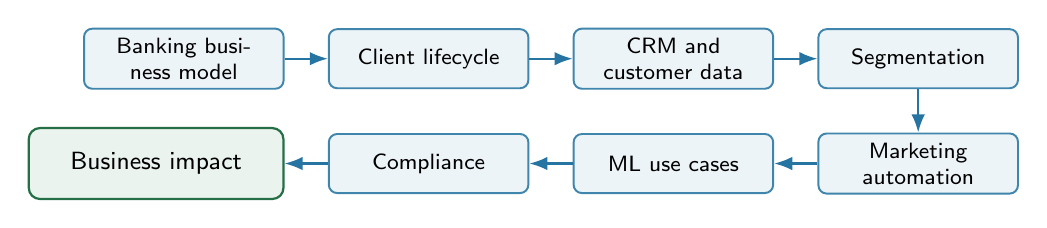
\begin{tikzpicture}[node distance=0.55cm]
	\node[smallflow] (b) {Banking business model};
	\node[smallflow, right=of b] (l) {Client lifecycle};
	\node[smallflow, right=of l] (crm) {CRM and customer data};
	\node[smallflow, right=of crm] (seg) {Segmentation};
	\node[smallflow, below=of seg] (auto) {Marketing automation};
	\node[smallflow, left=of auto] (ml) {ML use cases};
	\node[smallflow, left=of ml] (comp) {Compliance};
	\node[action, left=of comp] (impact) {Business impact};
	\draw[arrow] (b) -- (l);
	\draw[arrow] (l) -- (crm);
	\draw[arrow] (crm) -- (seg);
	\draw[arrow] (seg) -- (auto);
	\draw[arrow] (auto) -- (ml);
	\draw[arrow] (ml) -- (comp);
	\draw[arrow] (comp) -- (impact);
\end{tikzpicture}
\end{center}

\section{How to Use This PDF}

For each module, read the ``What it is'' and ``Why it matters'' first. Then redraw the diagram by hand. Finally answer the practical questions without looking at the text. If you can explain the integrated case study on Day 7, you have the right level of preparation for an internship conversation.

\chapterimage{header_study.jpg}
\chapter{One-Week Schedule}

\section{Daily Plan}

\begin{table}[H]
	\centering
	\begin{tabularx}{\textwidth}{L{0.12\textwidth} L{0.36\textwidth} Y}
		\toprule
		\textbf{Day} & \textbf{Focus} & \textbf{Main goal}\\
		\midrule
		Day 1 & Mediolanum and banking basics & Understand what the company does and how banks make money.\\
		Day 2 & Retail banking, wealth management, and bancassurance & Understand business lines and product families likely connected to campaigns.\\
		Day 3 & Client marketing, CRM, and customer lifecycle & Understand the operating context of Marketing Clienti.\\
		Day 4 & Segmentation, personalization, and marketing automation & Understand how campaigns are planned, targeted, executed, and measured.\\
		Day 5 & Data and machine learning in banking marketing & Understand the ML use cases closest to the internship.\\
		Day 6 & Compliance, governance, and explainability & Understand constraints around financial data, profiling, suitability, and model governance.\\
		Day 7 & Integration and case-study synthesis & Build a complete mental model of the role and prepare internship questions.\\
		\bottomrule
	\end{tabularx}
	\caption{One-week study schedule}
\end{table}

\section{Daily Output}

At the end of each day, write one page answering three prompts: what the business team is trying to achieve, what data is needed, and what could go wrong if the campaign or model is poorly governed. This converts passive reading into internship-ready judgment.

\begin{studybox}{Seven-Day Deliverable}
Create a final one-page explanation of this chain: client need, product relevance, CRM signal, segment, campaign action, Family Banker follow-up, compliance control, measurement, and business result.
\end{studybox}

\chapterimage{header_milan_skyline.jpg}
\chapter{Days 1-2: Mediolanum, Banking, and Products}

\section{Module 1 - Banca Mediolanum: Business Model and Strategic Context}

\moduleblock
{Banca Mediolanum is a bank-led financial services group built around retail clients, households, advisory relationships, digital channels, banking services, investments, insurance, and asset gathering. Its distinctive operating model is the Family Banker network combined with multi-channel service.}
{Marketing Clienti does not market isolated products in a vacuum. It supports a relationship model where client knowledge, advisor context, digital behavior, and product needs must be combined.}
{Family Banker, client-centric model, multi-channel banking, banking/investing/insurance offer, vertically integrated product manufacturing and distribution, households and affluent/private segments.}
{\source{Banca Mediolanum Investor Relations}{https://www.bancamediolanum.it/corporate/investors?lang=en}; \source{Q1 2026 press release}{https://www.bancamediolanum.it/static-assets/documenti/file/en/2026/05/07/CS_070526_ENG.pdf}; \source{Family Banker official site}{https://www.familybanker.it/}; \source{Business areas page}{https://www.bancamediolanum.it/aree-di-business}.}
{``Banca Mediolanum business model Family Banker''; ``Banca Mediolanum investor presentation client model''; ``Banca Mediolanum Family Banker network''.}
{Mediolanum business model map; traditional bank versus digital-only versus Mediolanum advisory-network model.}
{What does Mediolanum sell? Who are its clients? Why is the Family Banker network important? How does client marketing support the commercial network? Why is personalization strategically important?}
{A client has a salary account, a high cash balance, and no investment plan. Marketing Clienti can identify the need, provide educational content, and help the Family Banker prepare a compliant conversation.}
{\term{Family Banker}{the tied financial advisor relationship role}; \term{AUA/AUM}{assets under administration or management}; \term{multi-channel}{client service across advisors, digital, phone, and partner channels}; \term{asset gatherer}{a firm focused on attracting and retaining client financial assets}.}

\begin{figure}[H]
	\centering
	\resizebox{\textwidth}{!}{
	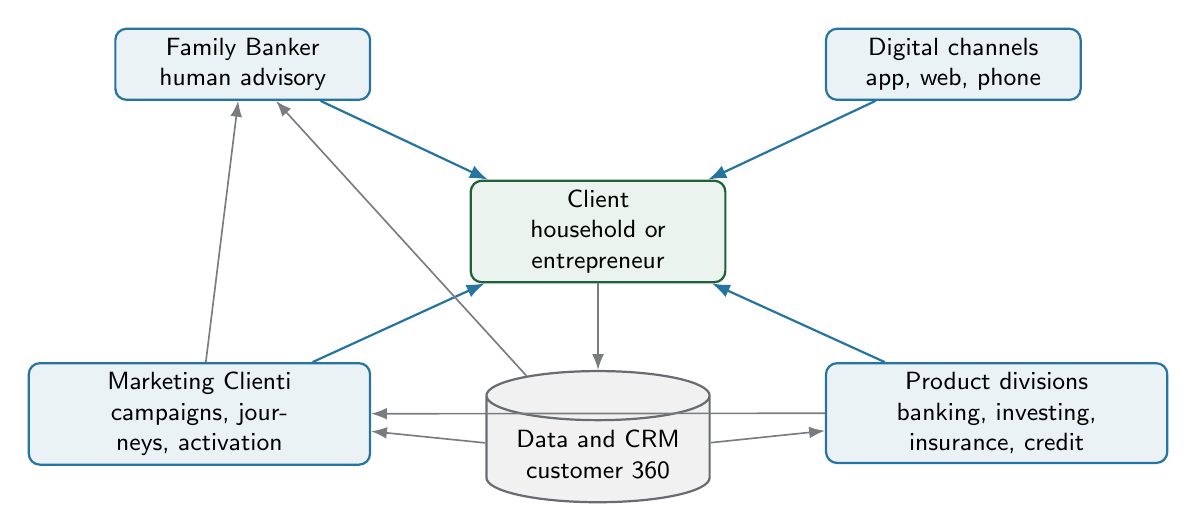
\begin{tikzpicture}[node distance=1.0cm and 1.25cm]
		\node[flow, fill=medgreen!10, draw=medgreen!70!black] (client) {Client\\household or entrepreneur};
		\node[flow, above left=of client] (fb) {Family Banker\\human advisory};
		\node[flow, above right=of client] (digital) {Digital channels\\app, web, phone};
		\node[wideflow, below left=of client] (marketing) {Marketing Clienti\\campaigns, journeys, activation};
		\node[wideflow, below right=of client] (products) {Product divisions\\banking, investing, insurance, credit};
		\node[data, below=1.1cm of client] (crm) {Data and CRM\\customer 360};
		\draw[arrow] (fb) -- (client);
		\draw[arrow] (digital) -- (client);
		\draw[arrow] (marketing) -- (client);
		\draw[arrow] (products) -- (client);
		\draw[softarrow] (client) -- (crm);
		\draw[softarrow] (crm) -- (marketing);
		\draw[softarrow] (crm) -- (fb);
		\draw[softarrow] (crm) -- (products);
		\draw[softarrow] (marketing) -- (fb);
		\draw[softarrow] (products) -- (marketing);
	\end{tikzpicture}}
	\caption{Mediolanum business model map}
\end{figure}

\begin{figure}[H]
	\centering
	\begin{tabularx}{\textwidth}{Y Y Y}
		\toprule
		\textbf{Traditional branch bank} & \textbf{Digital-only bank} & \textbf{Mediolanum advisory-network model}\\
		\midrule
		Branch-centric service, local physical presence, staff-led transactions. & App-centric self-service, low friction, low human advisory intensity. & Human advisor relationship plus direct digital service and centralized CRM/data support.\\
		Revenue often mixes lending spread, payments, fees, and branch-led sales. & Revenue often depends on scale, interchange, deposits, and selected lending. & Revenue emphasizes relationship depth, asset gathering, advisory, banking, investing, insurance, and retention.\\
		Marketing supports local and product campaigns. & Marketing supports digital acquisition and engagement. & Marketing supports both client communication and Family Banker enablement.\\
		\bottomrule
	\end{tabularx}
	\caption{Traditional bank versus Mediolanum model}
\end{figure}

\section{Module 2 - How Commercial Banks Make Money}

\moduleblock
{Commercial banks accept deposits, provide loans, manage payment services, hold securities, distribute financial products, and earn income from spreads and fees while managing liquidity, capital, and credit risk.}
{Marketing campaigns are judged by business impact. To understand impact, you must understand the difference between deposits, loans, asset management fees, insurance commissions, service fees, and retention economics.}
{Deposits, loans, net interest income, net interest margin, fee income, commissions, asset management fees, insurance distribution, capital, liquidity, credit risk, cost of risk.}
{\source{ECB educational explainers}{https://www.ecb.europa.eu/ecb/educational/pricestab/html/index.en.html}; \source{Bank of Italy financial education}{https://www.bancaditalia.it/compiti/tutela-educazione/educazione-finanziaria/index.html?com.dotmarketing.htmlpage.language=1}; \source{BBVA net interest income explainer}{https://www.bbva.com/en/economy-and-finance/what-does-a-banks-net-interest-income-include/}.}
{``how commercial banks make money net interest income commissions''; ``bank income statement net interest income net fee income''; ``ECB how banks work deposits loans capital''.}
{Bank balance sheet diagram; bank revenue model; client-to-bank money flow.}
{What is the difference between interest income and fee income? Why do banks care about deposits? Why are cross-selling and product adoption important? How do campaigns connect to revenue?}
{A campaign that attracts new liquidity can improve funding. A campaign that converts suitable clients into managed investments can create recurring fee income, but only after suitability and consent checks.}
{\term{Net interest income}{interest earned on assets minus interest paid on funding}; \term{NIM}{net interest margin}; \term{fee income}{commissions and service fees}; \term{cost of risk}{loan-loss cost relative to credit exposure}.}

\begin{figure}[H]
	\centering
	\resizebox{0.92\textwidth}{!}{
	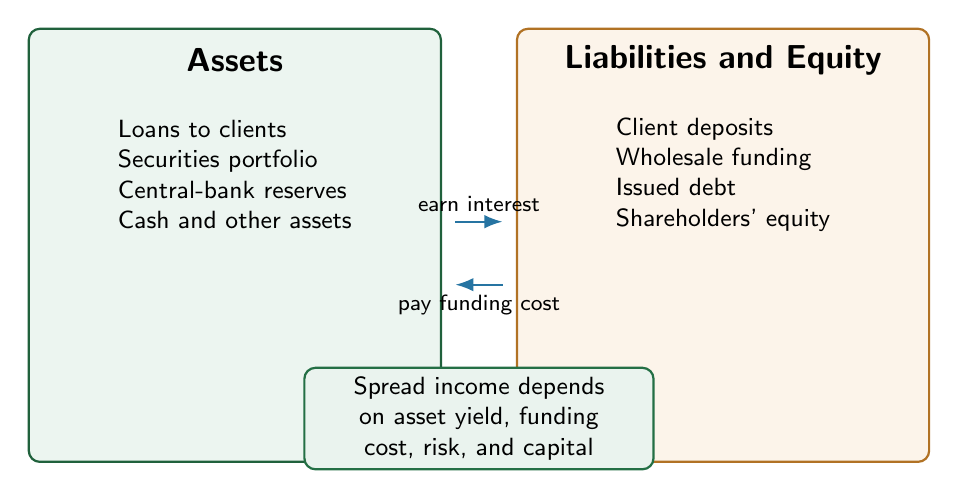
\begin{tikzpicture}
		\node[wideflow, fill=medgreen!9, draw=medgreen!70!black, minimum height=5.5cm, text width=5.0cm] (assets) at (0,0) {};
		\node[wideflow, fill=medamber!10, draw=medamber!80!black, minimum height=5.5cm, text width=5.0cm] (liab) at (6.2,0) {};
		\node[font=\sffamily\bfseries\large] at (0,2.35) {Assets};
		\node[font=\sffamily\bfseries\large] at (6.2,2.35) {Liabilities and Equity};
		\node[font=\sffamily\small, align=left] at (0,0.9) {Loans to clients\\Securities portfolio\\Central-bank reserves\\Cash and other assets};
		\node[font=\sffamily\small, align=left] at (6.2,0.9) {Client deposits\\Wholesale funding\\Issued debt\\Shareholders' equity};
		\draw[arrow] (2.8,0.3) -- node[above, font=\sffamily\footnotesize] {earn interest} (3.4,0.3);
		\draw[arrow] (3.4,-0.5) -- node[below, font=\sffamily\footnotesize] {pay funding cost} (2.8,-0.5);
		\node[action, text width=4.2cm] at (3.1,-2.2) {Spread income depends on asset yield, funding cost, risk, and capital};
	\end{tikzpicture}}
	\caption{Simplified bank balance sheet}
\end{figure}

\begin{figure}[H]
	\centering
	\resizebox{\textwidth}{!}{
	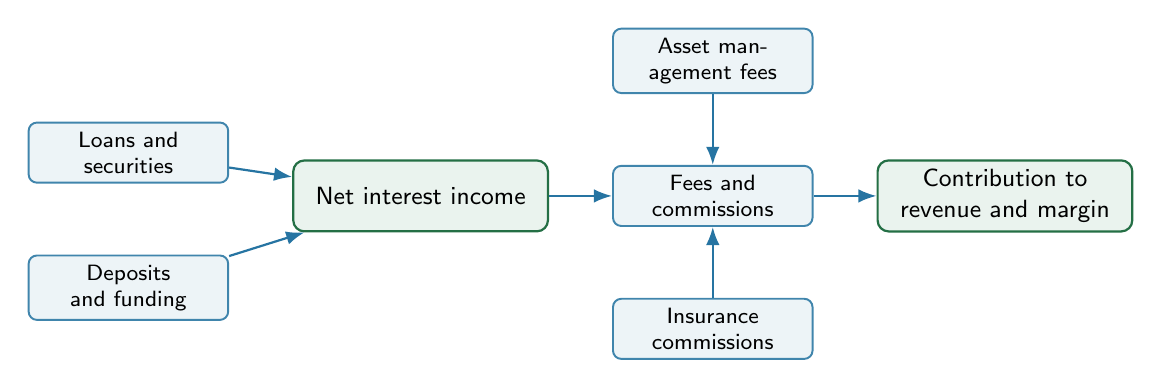
\begin{tikzpicture}[node distance=0.9cm and 0.8cm]
		\node[smallflow] (loans) {Loans and securities};
		\node[smallflow, below=of loans] (deposits) {Deposits and funding};
		\node[action, right=of loans, yshift=-0.55cm] (nii) {Net interest income};
		\node[smallflow, right=of nii] (fees) {Fees and commissions};
		\node[smallflow, above=of fees] (am) {Asset management fees};
		\node[smallflow, below=of fees] (ins) {Insurance commissions};
		\node[action, right=of fees] (profit) {Contribution to revenue and margin};
		\draw[arrow] (loans) -- (nii);
		\draw[arrow] (deposits) -- (nii);
		\draw[arrow] (nii) -- (fees);
		\draw[arrow] (am) -- (fees);
		\draw[arrow] (ins) -- (fees);
		\draw[arrow] (fees) -- (profit);
	\end{tikzpicture}}
	\caption{Bank revenue model}
\end{figure}

\section{Module 3 - Retail Banking, Wealth Management, and Bancassurance}

\moduleblock
{Retail banking covers everyday accounts, cards, payments, savings, mortgages, and personal loans. Wealth management covers investment advice, funds, managed portfolios, pensions, and planning. Bancassurance is the distribution of insurance through a bank relationship.}
{Client marketing campaigns often map to product families: onboarding a current account, encouraging digital activity, educating savers, supporting pension planning, or preparing an advisory conversation.}
{Current accounts, cards, mortgages, loans, savings, mutual funds, managed portfolios, pension products, life insurance, protection insurance, wealth management, private banking, bancassurance.}
{\source{Banca Mediolanum business areas}{https://www.bancamediolanum.it/aree-di-business}; \source{Family Banker advisory page}{https://www.familybanker.it/consulenza}; \source{Mediolanum Private Banking wealth management}{https://www.mediolanumprivatebanking.it/i-nostri-servizi/wealth-management}.}
{``Banca Mediolanum products accounts investments insurance pensions''; ``wealth management basics retail banking''; ``bancassurance explained''; ``retail banking products customer lifecycle''.}
{Product universe map; client lifecycle by product.}
{Which products are transactional? Which are advisory-based? Which generate recurring fees? Which require suitability checks?}
{A young client may start with a current account and card. Later signals such as recurring salary, cash accumulation, family events, or mortgage research can trigger educational journeys and advisor tasks.}
{\term{Bancassurance}{bank distribution of insurance products}; \term{managed assets}{assets placed in funds, mandates, or other managed solutions}; \term{suitability}{assessment that investment advice fits the client's knowledge, financial situation, objectives, risk tolerance, and sustainability preferences where relevant}.}

\begin{figure}[H]
	\centering
	\resizebox{\textwidth}{!}{
	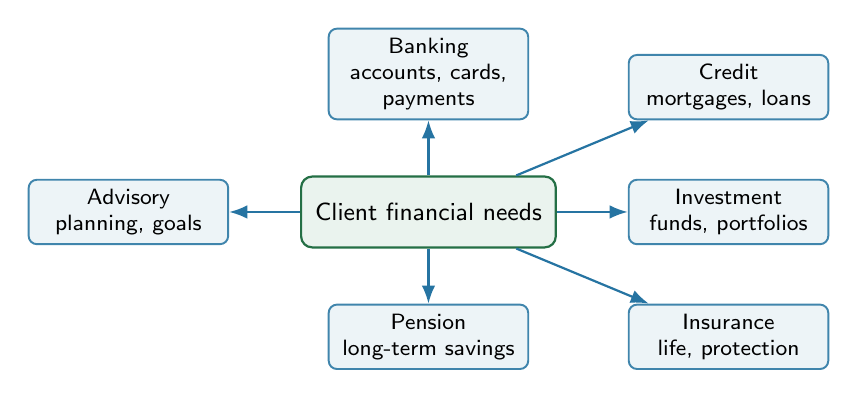
\begin{tikzpicture}[node distance=0.7cm and 0.9cm]
		\node[action, text width=3cm] (center) {Client financial needs};
		\node[smallflow, above=of center] (banking) {Banking\\accounts, cards, payments};
		\node[smallflow, above right=of center] (credit) {Credit\\mortgages, loans};
		\node[smallflow, right=of center] (invest) {Investment\\funds, portfolios};
		\node[smallflow, below right=of center] (insurance) {Insurance\\life, protection};
		\node[smallflow, below=of center] (pension) {Pension\\long-term savings};
		\node[smallflow, left=of center] (advice) {Advisory\\planning, goals};
		\foreach \x in {banking,credit,invest,insurance,pension,advice}{\draw[arrow] (center) -- (\x);}
	\end{tikzpicture}}
	\caption{Product universe map}
\end{figure}

\begin{figure}[H]
	\centering
	\resizebox{\textwidth}{!}{
	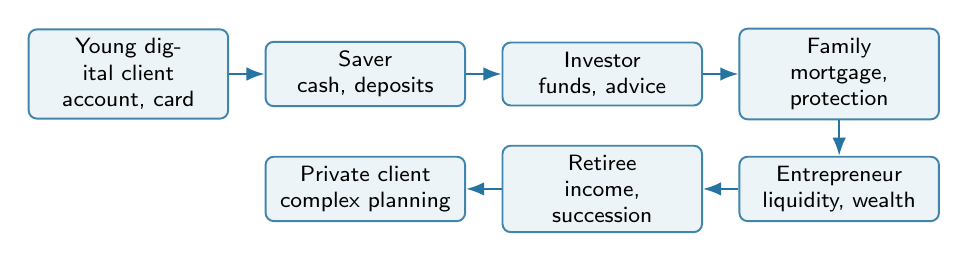
\begin{tikzpicture}[node distance=0.45cm]
		\node[smallflow] (young) {Young digital client\\account, card};
		\node[smallflow, right=of young] (saver) {Saver\\cash, deposits};
		\node[smallflow, right=of saver] (investor) {Investor\\funds, advice};
		\node[smallflow, right=of investor] (family) {Family\\mortgage, protection};
		\node[smallflow, below=of family] (entre) {Entrepreneur\\liquidity, wealth};
		\node[smallflow, left=of entre] (retire) {Retiree\\income, succession};
		\node[smallflow, left=of retire] (private) {Private client\\complex planning};
		\draw[arrow] (young) -- (saver);
		\draw[arrow] (saver) -- (investor);
		\draw[arrow] (investor) -- (family);
		\draw[arrow] (family) -- (entre);
		\draw[arrow] (entre) -- (retire);
		\draw[arrow] (retire) -- (private);
	\end{tikzpicture}}
	\caption{Client lifecycle by product}
\end{figure}

\chapterimage{header_business_meeting.jpg}
\chapter{Day 3: Organization, Client Marketing, and CRM}

\section{Module 4 - Organizational Structure and Stakeholders}

\moduleblock
{Marketing Clienti is one stakeholder in a broader bank operating model involving product teams, CRM, analytics, IT/data engineering, compliance, legal, risk, senior management, and the Family Banker network.}
{Most useful internship work requires translation across teams: business objective into data logic, data logic into campaign execution, and campaign results into clear business interpretation.}
{Campaign owner, product owner, data owner, CRM specialist, data scientist, IT/data engineering, compliance/legal, risk, Family Banker, senior management, client.}
{\source{Banca Mediolanum corporate governance}{https://www.bancamediolanum.it/corporate/investors?lang=en}; general bank operating model articles; CRM team responsibility resources; financial services marketing operating model resources.}
{``bank organizational structure retail banking marketing CRM compliance''; ``financial services marketing operating model CRM analytics''; ``bank marketing compliance data analytics collaboration''.}
{Stakeholder map; campaign approval workflow.}
{Who owns the client relationship? Who designs the campaign? Who owns the data? Who approves communications? Who evaluates success?}
{A pension education campaign requires product content, CRM targeting, consent rules, compliance review, Family Banker follow-up tasks, and measurement. No one team can complete it alone.}
{\term{RACI}{responsible, accountable, consulted, informed}; \term{campaign owner}{team accountable for campaign purpose and execution}; \term{data owner}{function accountable for data meaning and permitted use}; \term{approval workflow}{controlled path from idea to release}.}

\begin{figure}[H]
	\centering
	\resizebox{\textwidth}{!}{
	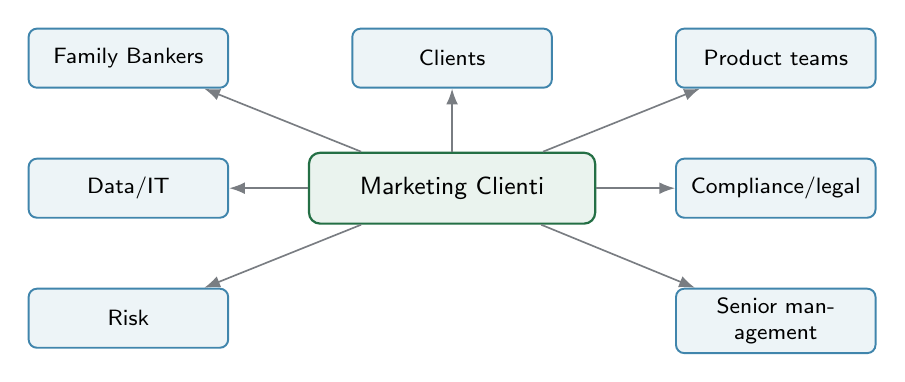
\begin{tikzpicture}[node distance=0.8cm and 1.0cm]
		\node[action, text width=3.4cm] (m) {Marketing Clienti};
		\node[smallflow, above=of m] (clients) {Clients};
		\node[smallflow, above left=of m] (fb) {Family Bankers};
		\node[smallflow, above right=of m] (prod) {Product teams};
		\node[smallflow, left=of m] (data) {Data/IT};
		\node[smallflow, right=of m] (comp) {Compliance/legal};
		\node[smallflow, below left=of m] (risk) {Risk};
		\node[smallflow, below right=of m] (mgmt) {Senior management};
		\foreach \x in {clients,fb,prod,data,comp,risk,mgmt}{\draw[softarrow] (m) -- (\x);}
	\end{tikzpicture}}
	\caption{Stakeholder map around Marketing Clienti}
\end{figure}

\begin{figure}[H]
	\centering
	\resizebox{\textwidth}{!}{
	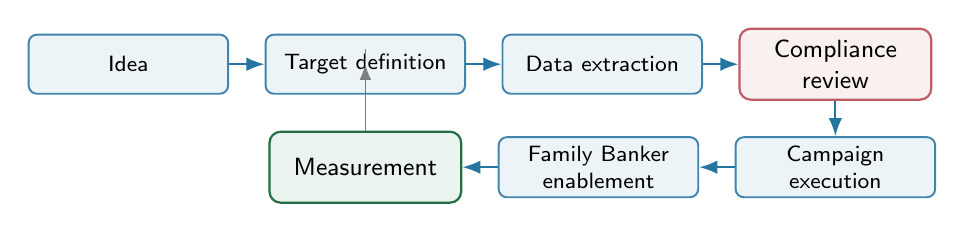
\begin{tikzpicture}[node distance=0.45cm]
		\node[smallflow] (idea) {Idea};
		\node[smallflow, right=of idea] (target) {Target definition};
		\node[smallflow, right=of target] (extract) {Data extraction};
		\node[risk, right=of extract, text width=2.2cm] (review) {Compliance review};
		\node[smallflow, below=of review] (exec) {Campaign execution};
		\node[smallflow, left=of exec] (fb) {Family Banker enablement};
		\node[action, left=of fb, text width=2.2cm] (measure) {Measurement};
		\draw[arrow] (idea) -- (target);
		\draw[arrow] (target) -- (extract);
		\draw[arrow] (extract) -- (review);
		\draw[arrow] (review) -- (exec);
		\draw[arrow] (exec) -- (fb);
		\draw[arrow] (fb) -- (measure);
		\draw[softarrow] (measure) |- (target);
	\end{tikzpicture}}
	\caption{Campaign approval workflow}
\end{figure}

\section{Module 5 - Client Marketing in Banking}

\moduleblock
{Client marketing manages communications and initiatives across acquisition, onboarding, engagement, development, cross-sell, retention, reactivation, education, events, and advisor enablement.}
{Bank marketing differs from consumer e-commerce because many products are regulated, high-trust, high-consideration, and relationship-based. The objective is not just a click; it is often a better conversation.}
{Acquisition, onboarding, development, retention, cross-selling, upselling, education, event marketing, reactivation, advisor support, commercial enablement, relationship depth.}
{Financial services lifecycle marketing guides; banking campaign case studies; CRM marketing resources; customer lifecycle materials from major CRM platforms.}
{``client marketing banking CRM lifecycle acquisition retention cross sell''; ``financial services customer lifecycle marketing''; ``banking cross-sell retention marketing automation''.}
{Bank customer lifecycle; client marketing funnel.}
{How is banking marketing different from consumer product marketing? Why is retention important? What is cross-selling in a bank? What campaigns might Mediolanum run?}
{A client who opened an account but never activated the app may receive onboarding nudges. The Family Banker may receive a task if the client is high value or needs personal help.}
{\term{Cross-sell}{encouraging adoption of an additional relevant product}; \term{retention}{keeping clients active and satisfied}; \term{relationship depth}{number and quality of products and interactions}; \term{enablement}{materials or tasks that help advisors act}.}

\begin{figure}[H]
	\centering
	\resizebox{\textwidth}{!}{
	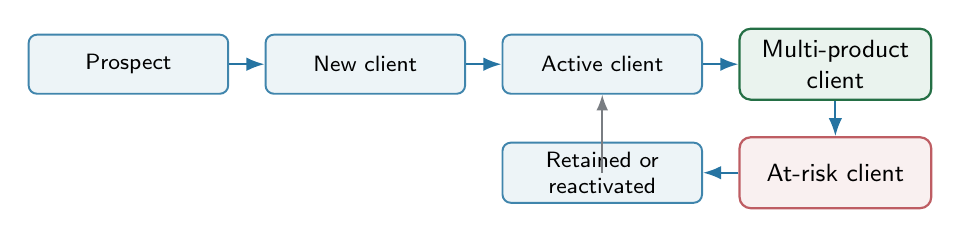
\begin{tikzpicture}[node distance=0.45cm]
		\node[smallflow] (p) {Prospect};
		\node[smallflow, right=of p] (n) {New client};
		\node[smallflow, right=of n] (a) {Active client};
		\node[action, right=of a, text width=2.2cm] (m) {Multi-product client};
		\node[risk, below=of m, text width=2.2cm] (r) {At-risk client};
		\node[smallflow, left=of r] (re) {Retained or reactivated};
		\draw[arrow] (p) -- (n);
		\draw[arrow] (n) -- (a);
		\draw[arrow] (a) -- (m);
		\draw[arrow] (m) -- (r);
		\draw[arrow] (r) -- (re);
		\draw[softarrow] (re) -| (a);
	\end{tikzpicture}}
	\caption{Bank customer lifecycle}
\end{figure}

\begin{figure}[H]
	\centering
	\resizebox{\textwidth}{!}{
	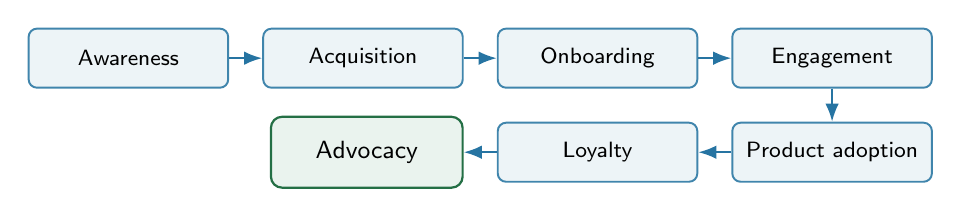
\begin{tikzpicture}[node distance=0.42cm]
		\node[smallflow] (aw) {Awareness};
		\node[smallflow, right=of aw] (acq) {Acquisition};
		\node[smallflow, right=of acq] (on) {Onboarding};
		\node[smallflow, right=of on] (eng) {Engagement};
		\node[smallflow, below=of eng] (adopt) {Product adoption};
		\node[smallflow, left=of adopt] (loy) {Loyalty};
		\node[action, left=of loy, text width=2.2cm] (adv) {Advocacy};
		\draw[arrow] (aw) -- (acq);
		\draw[arrow] (acq) -- (on);
		\draw[arrow] (on) -- (eng);
		\draw[arrow] (eng) -- (adopt);
		\draw[arrow] (adopt) -- (loy);
		\draw[arrow] (loy) -- (adv);
	\end{tikzpicture}}
	\caption{Client marketing funnel}
\end{figure}

\section{Module 6 - CRM Systems and Customer Data Models}

\moduleblock
{A CRM system stores and activates client relationship data: identity, accounts, product holdings, interactions, campaign history, consents, advisor relationships, leads, opportunities, events, preferences, and segments.}
{For a technical intern, CRM is where business intent becomes operational data. The same campaign idea can succeed or fail depending on entity definitions, data quality, consent, and integration.}
{Customer master data, product holdings, contact history, campaign history, consent management, interaction data, lead, opportunity, segment, event, communication preference, advisor relationship.}
{\source{Salesforce Customer 360 Data Model}{https://help.salesforce.com/s/articleView?id=data.c360_a_c360datamodel.htm}; \source{Salesforce Financial Services data model}{https://developer.salesforce.com/docs/platform/data-models/guide/data-cloud-financial-services-overview.html}; customer data platform documentation.}
{``CRM data model customer 360 banking''; ``financial services CRM data model''; ``customer 360 data model financial services''; ``CRM campaign history contact history data model''.}
{CRM entity-relationship diagram; customer 360 view.}
{What does a CRM store? What is a customer 360? Why is consent important? What is campaign history? How does CRM data become ML-ready?}
{If a client opted out of email but permits app notifications, the CRM must expose that preference before a journey is launched. Otherwise the campaign is not operationally usable.}
{\term{Customer 360}{unified operational view of a client}; \term{contact history}{record of outbound and inbound interactions}; \term{consent}{permission or legal basis signal for communication and data use}; \term{golden record}{trusted master identity record}.}

\begin{figure}[H]
	\centering
	\resizebox{\textwidth}{!}{
	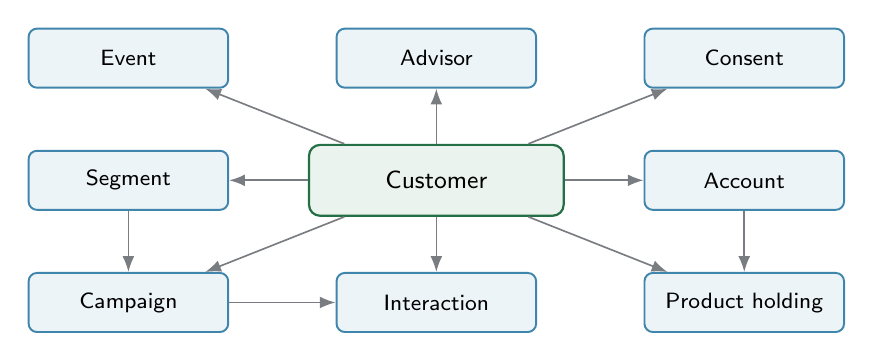
\begin{tikzpicture}[node distance=0.7cm and 1.0cm]
		\node[action] (cust) {Customer};
		\node[smallflow, above=of cust] (advisor) {Advisor};
		\node[smallflow, above right=of cust] (consent) {Consent};
		\node[smallflow, right=of cust] (account) {Account};
		\node[smallflow, below right=of cust] (product) {Product holding};
		\node[smallflow, below=of cust] (interaction) {Interaction};
		\node[smallflow, below left=of cust] (campaign) {Campaign};
		\node[smallflow, left=of cust] (segment) {Segment};
		\node[smallflow, above left=of cust] (event) {Event};
		\foreach \x in {advisor,consent,account,product,interaction,campaign,segment,event}{\draw[softarrow] (cust) -- (\x);}
		\draw[softarrow] (campaign) -- (interaction);
		\draw[softarrow] (segment) -- (campaign);
		\draw[softarrow] (account) -- (product);
	\end{tikzpicture}}
	\caption{Simplified CRM entity-relationship diagram}
\end{figure}

\begin{figure}[H]
	\centering
	\resizebox{\textwidth}{!}{
	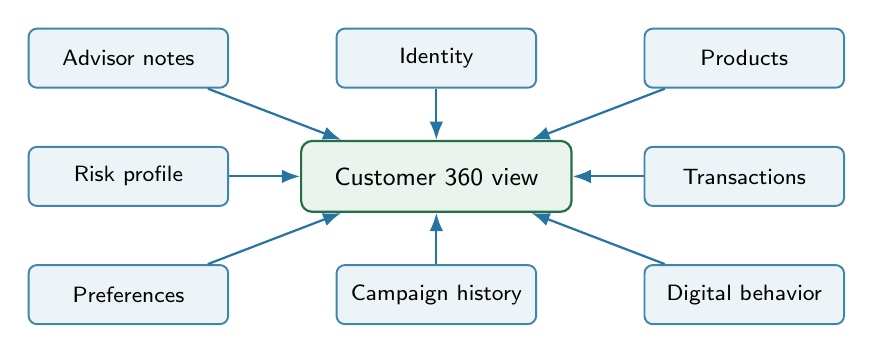
\begin{tikzpicture}[node distance=0.65cm and 0.9cm]
		\node[action, text width=3.2cm] (c) {Customer 360 view};
		\node[smallflow, above=of c] (id) {Identity};
		\node[smallflow, above right=of c] (prod) {Products};
		\node[smallflow, right=of c] (tx) {Transactions};
		\node[smallflow, below right=of c] (dig) {Digital behavior};
		\node[smallflow, below=of c] (hist) {Campaign history};
		\node[smallflow, below left=of c] (pref) {Preferences};
		\node[smallflow, left=of c] (risk) {Risk profile};
		\node[smallflow, above left=of c] (notes) {Advisor notes};
		\foreach \x in {id,prod,tx,dig,hist,pref,risk,notes}{\draw[arrow] (\x) -- (c);}
	\end{tikzpicture}}
	\caption{Customer 360 view}
\end{figure}

\chapterimage{header_analytics_dashboard.jpg}
\chapter{Day 4: Segmentation, Personalization, and Automation}

\section{Module 7 - Segmentation and Personalization}

\moduleblock
{Segmentation groups clients into actionable sets based on demographic, behavioral, financial, needs-based, life-stage, value-based, or predictive signals. Personalization adapts message, channel, timing, and advisor action to the segment or client.}
{Segmentation is the bridge between raw customer data and useful campaigns. It decides who should receive a message, who should be suppressed, and what the Family Banker should know.}
{Demographic segmentation, behavioral segmentation, financial segmentation, needs-based segmentation, life-stage segmentation, RFM, clustering, lookalike audiences, personalization rules, suitability constraints.}
{Banking segmentation guides; RFM tutorials; clustering tutorials; financial services customer segmentation papers; personas in banking case studies.}
{``banking customer segmentation models''; ``financial services customer segmentation machine learning''; ``RFM analysis customer segmentation banking''; ``customer segmentation clustering tutorial''.}
{Segmentation pyramid; example client segments; segmentation-to-campaign flow.}
{Why is segmentation useful? What is the difference between rule-based and ML-based segmentation? What makes a segment actionable? How do you avoid inappropriate targeting?}
{High-liquidity savers are not automatically investment prospects. The segment becomes actionable only after consent, risk profile, existing holdings, recent communications, and advisor context are checked.}
{\term{RFM}{recency, frequency, monetary value}; \term{cluster}{group discovered from data similarity}; \term{persona}{human-readable archetype}; \term{actionability}{ability to link a segment to a compliant business action}.}

\begin{figure}[H]
	\centering
	\resizebox{0.78\textwidth}{!}{
	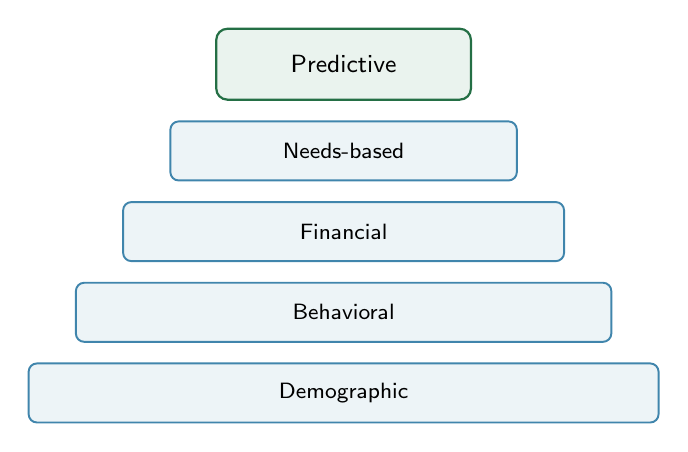
\begin{tikzpicture}
		\node[smallflow, minimum width=8.0cm] (demo) at (0,0) {Demographic};
		\node[smallflow, minimum width=6.8cm, above=0.25cm of demo] (beh) {Behavioral};
		\node[smallflow, minimum width=5.6cm, above=0.25cm of beh] (fin) {Financial};
		\node[smallflow, minimum width=4.4cm, above=0.25cm of fin] (needs) {Needs-based};
		\node[action, minimum width=3.2cm, above=0.25cm of needs] (pred) {Predictive};
	\end{tikzpicture}}
	\caption{Segmentation pyramid}
\end{figure}

\begin{figure}[H]
	\centering
	\begin{tabularx}{\textwidth}{L{0.25\textwidth} Y Y}
		\toprule
		\textbf{Example segment} & \textbf{Signal} & \textbf{Possible campaign}\\
		\midrule
		Young digital client & Mobile-heavy activity, few products & App onboarding and card usage education.\\
		High-liquidity saver & Large current account balance, low investment adoption & Financial planning education and advisor prompt.\\
		New investor & Recent first fund purchase & Risk education, periodic investing material, meeting follow-up.\\
		Family planning client & Mortgage research, child-related life stage signals & Protection and long-term planning education.\\
		Retirement-focused client & Age and pension interest & Pension review journey and advisor preparation.\\
		Inactive client & Low login, no recent interaction & Reactivation with low-frequency outreach.\\
		\bottomrule
	\end{tabularx}
	\caption{Example client segments}
\end{figure}

\begin{figure}[H]
	\centering
	\resizebox{\textwidth}{!}{
	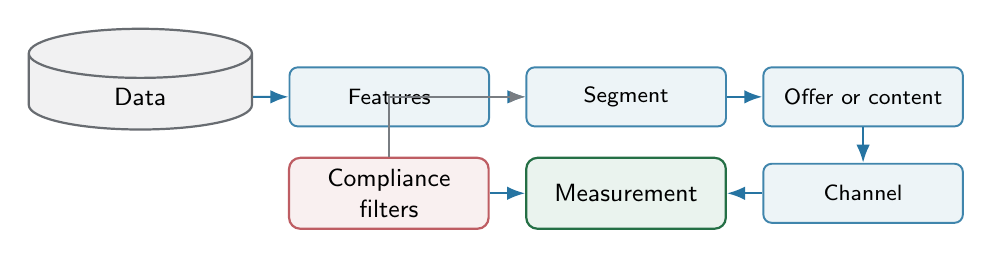
\begin{tikzpicture}[node distance=0.45cm]
		\node[data] (data) {Data};
		\node[smallflow, right=of data] (features) {Features};
		\node[smallflow, right=of features] (segment) {Segment};
		\node[smallflow, right=of segment] (offer) {Offer or content};
		\node[smallflow, below=of offer] (channel) {Channel};
		\node[action, left=of channel, text width=2.3cm] (measure) {Measurement};
		\node[risk, left=of measure, text width=2.3cm] (filters) {Compliance filters};
		\draw[arrow] (data) -- (features);
		\draw[arrow] (features) -- (segment);
		\draw[arrow] (segment) -- (offer);
		\draw[arrow] (offer) -- (channel);
		\draw[arrow] (channel) -- (measure);
		\draw[arrow] (filters) -- (measure);
		\draw[softarrow] (filters) |- (segment);
	\end{tikzpicture}}
	\caption{Segmentation-to-campaign flow}
\end{figure}

\section{Module 8 - Marketing Automation and Campaign Management}

\moduleblock
{Marketing automation coordinates audience selection, triggers, journeys, channels, suppression rules, frequency caps, advisor tasks, A/B tests, campaign calendars, tracking, attribution, and feedback into CRM.}
{The internship may involve campaign logic, data extracts, journey rules, dashboards, or model scores. Automation turns strategy into repeatable execution.}
{Campaign planning, audience selection, triggers, journeys, email, SMS, app notifications, advisor tasks, channel coordination, A/B testing, suppression rules, frequency caps, attribution, real-time metrics.}
{\source{Oracle Eloqua marketing automation docs}{https://docs.oracle.com/en/cloud/saas/marketing/eloqua.html}; \source{Salesforce Data 360 integration patterns}{https://architect.salesforce.com/docs/architect/fundamentals/guide/data360_integration_patterns_and_practices.html}; customer journey orchestration resources.}
{``marketing automation banking customer journey CRM''; ``customer journey orchestration financial services''; ``campaign management process CRM''; ``A/B testing marketing campaigns banking''.}
{Campaign execution pipeline; triggered journey example.}
{What is marketing automation? What is a customer journey? What is the difference between batch and triggered campaigns? How do campaigns interact with advisors?}
{A high-liquidity trigger creates an educational app message. If the client engages, a Family Banker task is created. If there was recent outreach, a frequency cap suppresses the next contact.}
{\term{Journey}{sequence of messages and decisions over time}; \term{trigger}{event that starts or changes a journey}; \term{suppression}{rule that excludes a client}; \term{frequency cap}{limit on communication volume}.}

\begin{figure}[H]
	\centering
	\resizebox{\textwidth}{!}{
	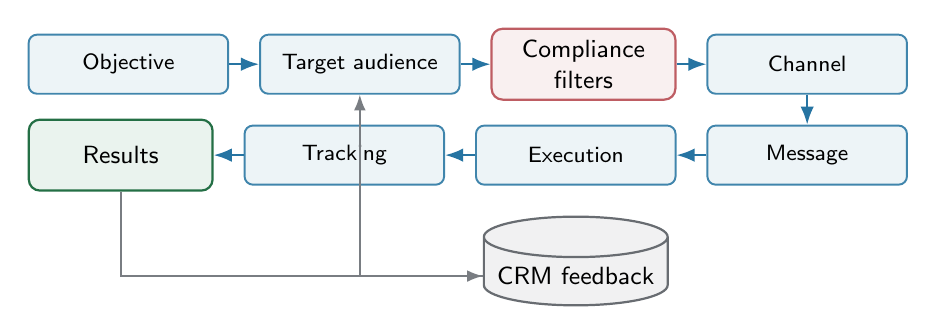
\begin{tikzpicture}[node distance=0.38cm]
		\node[smallflow] (obj) {Objective};
		\node[smallflow, right=of obj] (target) {Target audience};
		\node[risk, right=of target, text width=2.1cm] (filter) {Compliance filters};
		\node[smallflow, right=of filter] (channel) {Channel};
		\node[smallflow, below=of channel] (msg) {Message};
		\node[smallflow, left=of msg] (exec) {Execution};
		\node[smallflow, left=of exec] (track) {Tracking};
		\node[action, left=of track, text width=2.1cm] (results) {Results};
		\node[data, below=of exec, text width=2.1cm] (crm) {CRM feedback};
		\draw[arrow] (obj) -- (target);
		\draw[arrow] (target) -- (filter);
		\draw[arrow] (filter) -- (channel);
		\draw[arrow] (channel) -- (msg);
		\draw[arrow] (msg) -- (exec);
		\draw[arrow] (exec) -- (track);
		\draw[arrow] (track) -- (results);
		\draw[softarrow] (results) |- (crm);
		\draw[softarrow] (crm) -| (target);
	\end{tikzpicture}}
	\caption{Marketing automation pipeline}
\end{figure}

\begin{figure}[H]
	\centering
	\resizebox{\textwidth}{!}{
	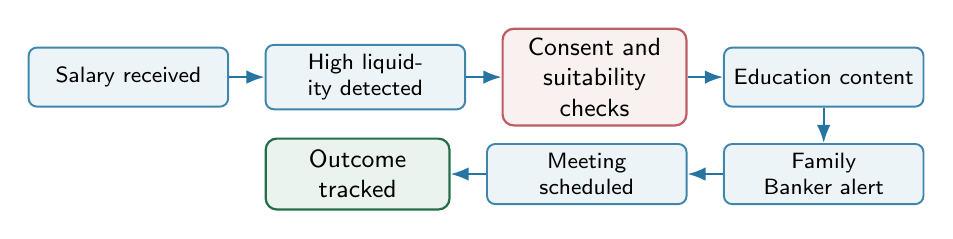
\begin{tikzpicture}[node distance=0.45cm]
		\node[smallflow] (salary) {Salary received};
		\node[smallflow, right=of salary] (liq) {High liquidity detected};
		\node[risk, right=of liq, text width=2.1cm] (rules) {Consent and suitability checks};
		\node[smallflow, right=of rules] (edu) {Education content};
		\node[smallflow, below=of edu] (alert) {Family Banker alert};
		\node[smallflow, left=of alert] (meet) {Meeting scheduled};
		\node[action, left=of meet, text width=2.1cm] (outcome) {Outcome tracked};
		\draw[arrow] (salary) -- (liq);
		\draw[arrow] (liq) -- (rules);
		\draw[arrow] (rules) -- (edu);
		\draw[arrow] (edu) -- (alert);
		\draw[arrow] (alert) -- (meet);
		\draw[arrow] (meet) -- (outcome);
	\end{tikzpicture}}
	\caption{Triggered journey example}
\end{figure}

\chapterimage{header_data_center.jpg}
\chapter{Day 5: Machine Learning and Data Pipelines}

\section{Module 9 - Machine Learning Use Cases in Client Marketing}

\moduleblock
{Machine learning in client marketing predicts or scores useful business signals: churn risk, response propensity, next best action, lead quality, product relevance, lifetime value, uplift, channel preference, send time, segment membership, and interaction themes.}
{The business value of ML is not the model itself. Value appears only when scores are delivered into campaigns, advisor tools, dashboards, and decisions that teams trust and can explain.}
{Churn prediction, propensity modeling, next best action, lead scoring, product recommendation, CLV, response prediction, uplift modeling, channel preference, send-time optimization, clustering, NLP, explainability.}
{\source{Retail banking churn prediction paper}{https://link.springer.com/article/10.1186/s40854-023-00558-3}; \source{Retail banking CLV paper}{https://arxiv.org/abs/2304.03038}; \source{scikit-uplift documentation}{https://www.uplift-modeling.com/en/latest/user_guide/index.html}; explainable AI resources.}
{``machine learning CRM banking churn prediction propensity model''; ``next best action banking machine learning''; ``uplift modeling marketing campaigns tutorial''; ``customer lifetime value prediction banking machine learning''.}
{ML use case matrix; propensity model workflow; next-best-action architecture.}
{What is a propensity model? What is the difference between prediction and recommendation? Why is uplift modeling useful? Why does explainability matter?}
{A propensity model ranks clients likely to schedule an investment conversation after an education campaign. It should not decide suitability or replace the Family Banker.}
{\term{Propensity}{probability of a future behavior}; \term{uplift}{incremental effect caused by a treatment}; \term{CLV}{customer lifetime value}; \term{NBA}{next best action}; \term{XAI}{explainable AI}.}

\begin{table}[H]
	\centering
	\footnotesize
	\begin{tabularx}{\textwidth}{L{0.15\textwidth} L{0.20\textwidth} L{0.16\textwidth} L{0.16\textwidth} Y}
		\toprule
		\textbf{Use case} & \textbf{Input data} & \textbf{Model type} & \textbf{Output} & \textbf{Business action and risk}\\
		\midrule
		Churn & inactivity, product changes, complaints & classification & churn risk score & retention task; risk of over-contacting.\\
		Propensity & history, holdings, engagement & classification/ranking & likelihood to respond & target campaign; risk of proxy bias.\\
		Next best action & CRM, rules, scores, constraints & recommender/rules + ML & ranked action & advisor suggestion; risk of unsuitable recommendation.\\
		CLV & balances, products, fees, tenure & regression/survival & future value & prioritization; risk of unfair service allocation.\\
		Uplift & randomized campaign outcomes & causal ML/meta-learners & incremental effect & target persuadable clients; risk of weak experiment design.\\
		\bottomrule
	\end{tabularx}
	\caption{ML use case matrix for client marketing}
\end{table}

\begin{figure}[H]
	\centering
	\resizebox{\textwidth}{!}{
	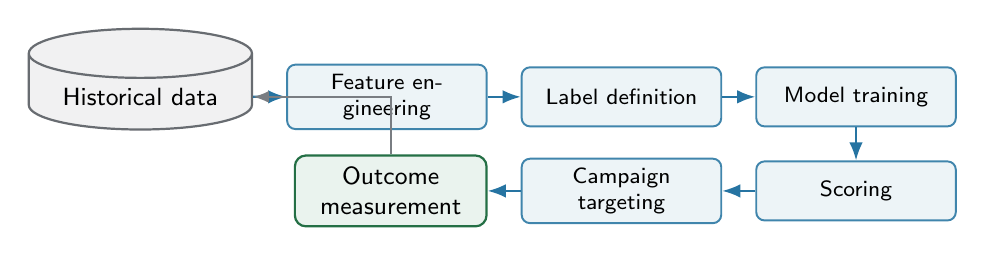
\begin{tikzpicture}[node distance=0.42cm]
		\node[data] (hist) {Historical data};
		\node[smallflow, right=of hist] (feat) {Feature engineering};
		\node[smallflow, right=of feat] (label) {Label definition};
		\node[smallflow, right=of label] (train) {Model training};
		\node[smallflow, below=of train] (score) {Scoring};
		\node[smallflow, left=of score] (target) {Campaign targeting};
		\node[action, left=of target, text width=2.2cm] (measure) {Outcome measurement};
		\draw[arrow] (hist) -- (feat);
		\draw[arrow] (feat) -- (label);
		\draw[arrow] (label) -- (train);
		\draw[arrow] (train) -- (score);
		\draw[arrow] (score) -- (target);
		\draw[arrow] (target) -- (measure);
		\draw[softarrow] (measure) |- (hist);
	\end{tikzpicture}}
	\caption{Propensity model workflow}
\end{figure}

\begin{figure}[H]
	\centering
	\resizebox{\textwidth}{!}{
	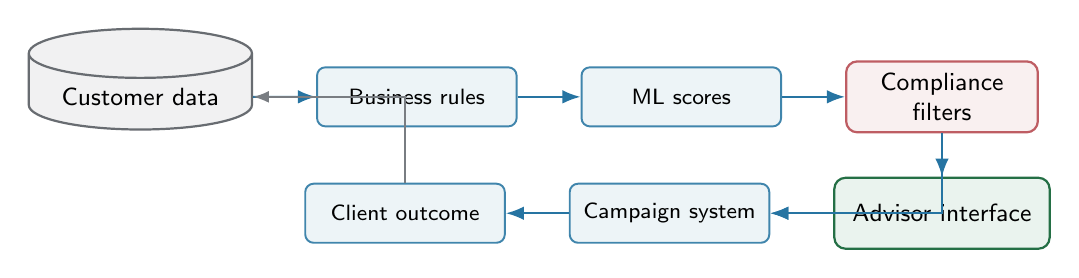
\begin{tikzpicture}[node distance=0.55cm and 0.8cm]
		\node[data] (cust) {Customer data};
		\node[smallflow, right=of cust] (rules) {Business rules};
		\node[smallflow, right=of rules] (scores) {ML scores};
		\node[risk, right=of scores, text width=2.2cm] (filters) {Compliance filters};
		\node[action, below=of filters, text width=2.5cm] (advisor) {Advisor interface};
		\node[smallflow, left=of advisor] (campaign) {Campaign system};
		\node[smallflow, left=of campaign] (outcome) {Client outcome};
		\draw[arrow] (cust) -- (rules);
		\draw[arrow] (rules) -- (scores);
		\draw[arrow] (scores) -- (filters);
		\draw[arrow] (filters) -- (advisor);
		\draw[arrow] (filters) |- (campaign);
		\draw[arrow] (advisor) -- (campaign);
		\draw[arrow] (campaign) -- (outcome);
		\draw[softarrow] (outcome) |- (cust);
	\end{tikzpicture}}
	\caption{Next-best-action architecture}
\end{figure}

\section{Module 10 - Data Engineering and Analytics Pipeline}

\moduleblock
{A data pipeline moves data from source systems into analytical and operational environments: ETL/ELT, warehouse, customer data platform, feature creation, batch or real-time scoring, dashboards, monitoring, and activation back into CRM.}
{An intern may be asked to analyze campaign performance, prepare features, debug inconsistent data, document a flow, or support automation. Understanding data lineage prevents wrong conclusions.}
{Source systems, ETL/ELT, data warehouse, customer data platform, feature store, batch scoring, real-time scoring, dashboards, model monitoring, data quality, MDM, identity resolution.}
{\source{Salesforce Data 360 architecture}{https://architect.salesforce.com/docs/architect/fundamentals/guide/data-360-architecture}; \source{BCBS 239 risk data aggregation principles}{https://www.bis.org/publ/bcbs239.htm}; feature store tutorials; analytics engineering resources.}
{``customer data platform financial services architecture''; ``CRM analytics data pipeline architecture''; ``machine learning pipeline customer propensity scoring''; ``data quality customer 360 banking''.}
{End-to-end data architecture; batch scoring versus real-time scoring.}
{Where does the data come from? How does raw data become features? How are model outputs delivered to business users? What data quality issues matter most?}
{A model score is useless if it arrives after the campaign deadline, if customer IDs do not match CRM IDs, or if consent status is stale.}
{\term{ETL/ELT}{extract, transform, load or extract, load, transform}; \term{feature}{model-ready variable}; \term{lineage}{trace from output back to source}; \term{MDM}{master data management}; \term{identity resolution}{linking records that represent the same person}.}

\begin{figure}[H]
	\centering
	\resizebox{\textwidth}{!}{
	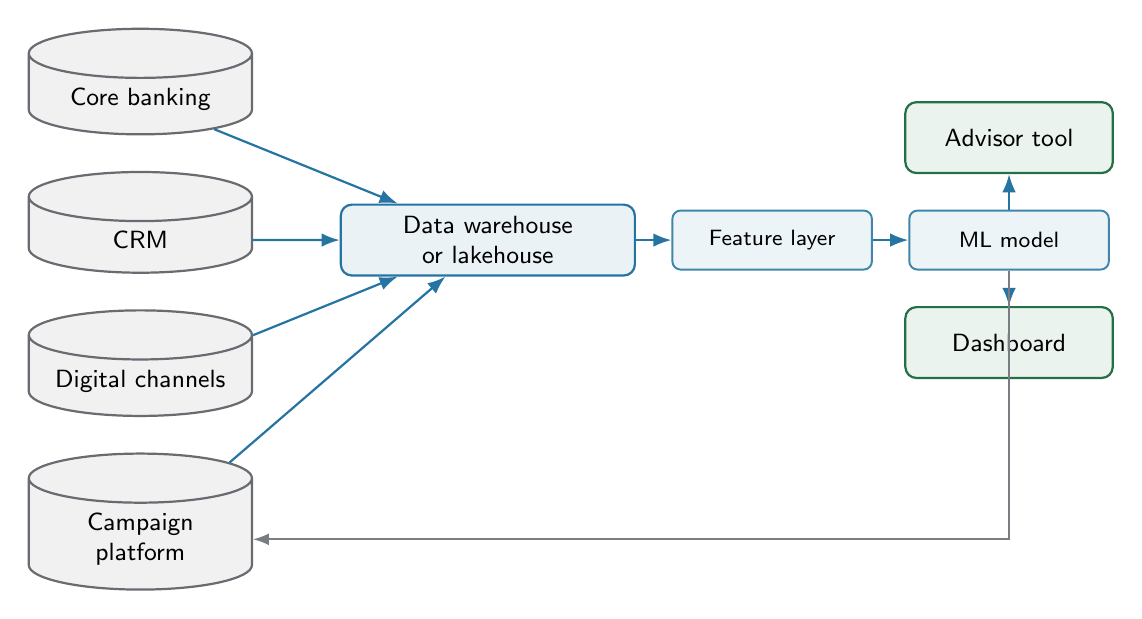
\begin{tikzpicture}[node distance=0.45cm]
		\node[data] (core) {Core banking};
		\node[data, below=of core] (crm) {CRM};
		\node[data, below=of crm] (digital) {Digital channels};
		\node[data, below=of digital] (campaign) {Campaign platform};
		\node[wideflow, right=1.1cm of crm, text width=3.5cm] (dw) {Data warehouse or lakehouse};
		\node[smallflow, right=of dw] (features) {Feature layer};
		\node[smallflow, right=of features] (model) {ML model};
		\node[action, below=of model, text width=2.4cm] (dash) {Dashboard};
		\node[action, above=of model, text width=2.4cm] (advisor) {Advisor tool};
		\draw[arrow] (core) -- (dw);
		\draw[arrow] (crm) -- (dw);
		\draw[arrow] (digital) -- (dw);
		\draw[arrow] (campaign) -- (dw);
		\draw[arrow] (dw) -- (features);
		\draw[arrow] (features) -- (model);
		\draw[arrow] (model) -- (dash);
		\draw[arrow] (model) -- (advisor);
		\draw[softarrow] (model) |- (campaign);
	\end{tikzpicture}}
	\caption{Data architecture for CRM and ML}
\end{figure}

\begin{figure}[H]
	\centering
	\begin{tabularx}{\textwidth}{Y Y}
		\toprule
		\textbf{Batch scoring} & \textbf{Real-time scoring}\\
		\midrule
		Scores are computed on a schedule, for example nightly or weekly. Best for planned campaigns, regular prioritization, churn lists, and dashboard refreshes. & Scores are computed or retrieved when an event happens, for example a login, salary credit, product page visit, or advisor interaction. Best for triggered journeys and in-session recommendations.\\
		Lower operational complexity and easier governance. & Higher integration complexity and stricter latency, monitoring, and fallback requirements.\\
		\bottomrule
	\end{tabularx}
	\caption{Batch scoring versus real-time scoring}
\end{figure}

\chapterimage{header_eu_parliament.jpg}
\chapter{Day 6: Metrics, Experimentation, Compliance, and Governance}

\section{Module 11 - Metrics, Experimentation, and Business Impact}

\moduleblock
{Marketing and ML work is evaluated with operational metrics, engagement metrics, business metrics, and incremental impact. A campaign is not successful just because it generated opens or clicks.}
{Business stakeholders care whether work improves client outcomes, supports Family Bankers, increases suitable conversations, reduces churn, grows assets, improves retention, or creates measurable incremental value.}
{Conversion rate, response rate, open rate, click-through rate, churn rate, retention rate, cross-sell rate, ROI, net inflows, CLV, CPA, incrementality, A/B testing, holdout groups, uplift, attribution.}
{Marketing analytics tutorials; A/B testing resources; uplift modeling resources; banking KPI resources; customer lifetime value resources.}
{``marketing campaign metrics conversion churn retention cross sell''; ``A/B testing marketing campaigns holdout group incrementality''; ``campaign attribution financial services''; ``uplift modeling campaign measurement''.}
{Campaign measurement framework; metrics hierarchy.}
{Why are clicks not enough? What is incrementality? Why do you need a control group? What is a good campaign metric in banking?}
{A campaign produces many opens but no extra meetings versus the holdout group. The business interpretation should be that the content drew attention but did not create incremental commercial action.}
{\term{Incrementality}{outcome caused by the campaign above what would have happened anyway}; \term{holdout}{similar group intentionally not exposed}; \term{attribution}{assigning credit for outcomes}; \term{ROI}{return on investment}.}

\begin{figure}[H]
	\centering
	\resizebox{\textwidth}{!}{
	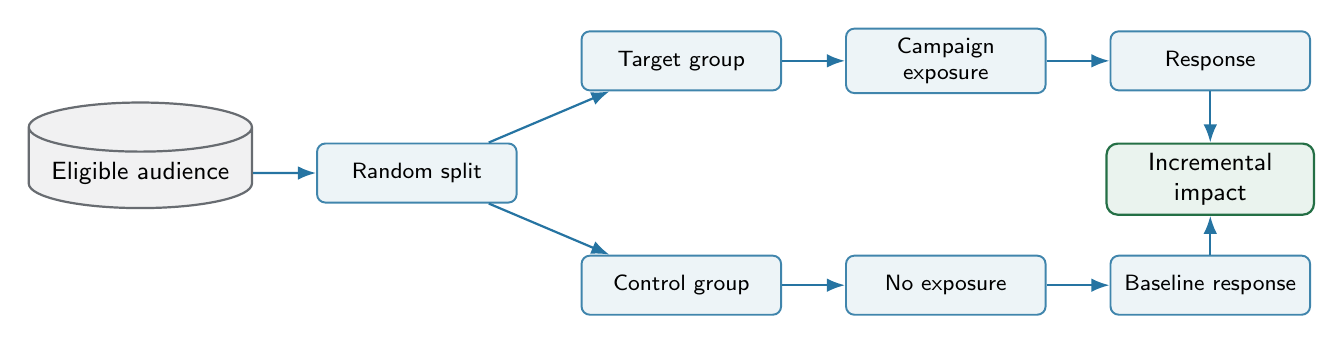
\begin{tikzpicture}[node distance=0.65cm and 0.8cm]
		\node[data] (eligible) {Eligible audience};
		\node[smallflow, right=of eligible] (split) {Random split};
		\node[smallflow, above right=of split] (target) {Target group};
		\node[smallflow, below right=of split] (control) {Control group};
		\node[smallflow, right=of target] (expose) {Campaign exposure};
		\node[smallflow, right=of expose] (resp) {Response};
		\node[action, below=of resp, text width=2.4cm] (impact) {Incremental impact};
		\node[smallflow, right=of control] (no) {No exposure};
		\node[smallflow, right=of no] (base) {Baseline response};
		\draw[arrow] (eligible) -- (split);
		\draw[arrow] (split) -- (target);
		\draw[arrow] (split) -- (control);
		\draw[arrow] (target) -- (expose);
		\draw[arrow] (expose) -- (resp);
		\draw[arrow] (control) -- (no);
		\draw[arrow] (no) -- (base);
		\draw[arrow] (resp) -- (impact);
		\draw[arrow] (base) -- (impact);
	\end{tikzpicture}}
	\caption{Campaign measurement framework}
\end{figure}

\begin{figure}[H]
	\centering
	\resizebox{0.9\textwidth}{!}{
	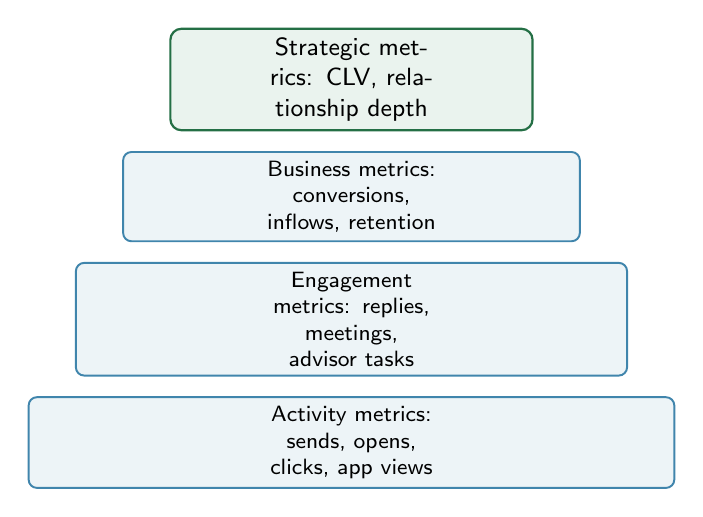
\begin{tikzpicture}
		\node[smallflow, minimum width=8.2cm] (activity) at (0,0) {Activity metrics: sends, opens, clicks, app views};
		\node[smallflow, minimum width=7.0cm, above=0.25cm of activity] (engage) {Engagement metrics: replies, meetings, advisor tasks};
		\node[smallflow, minimum width=5.8cm, above=0.25cm of engage] (business) {Business metrics: conversions, inflows, retention};
		\node[action, minimum width=4.6cm, above=0.25cm of business] (strategic) {Strategic metrics: CLV, relationship depth};
	\end{tikzpicture}}
	\caption{Metrics hierarchy}
\end{figure}

\section{Module 12 - Compliance, Privacy, and Model Governance}

\moduleblock
{Banking marketing uses personal and financial data under strict rules: GDPR, consent, profiling limits, data minimization, MiFID II suitability, KYC, AML, auditability, model governance, fairness, explainability, data retention, and human review.}
{The safest technical solution is not always the most predictive one. In financial services, data use must be lawful, proportionate, explainable, auditable, and aligned with client protection.}
{GDPR, consent, profiling, automated decision-making, data minimization, MiFID II suitability, KYC, AML, auditability, model risk management, bias, fairness, human-in-the-loop, explainability, retention.}
{\source{EDPB automated decision-making and profiling guidance}{https://www.edpb.europa.eu/our-work-tools/our-documents/guidelines/automated-decision-making-and-profiling_en}; \source{ESMA MiFID II suitability guidelines}{https://www.esma.europa.eu/document/guidelines-certain-aspects-mifid-ii-suitability-requirements-1}; \source{EBA Big Data and Advanced Analytics report}{https://eba.europa.eu/publications-and-media/press-releases/eba-report-identifies-key-challenges-roll-out-big-data-and}; \source{European Commission AI Act overview}{https://commission.europa.eu/news/ai-act-enters-force-2024-08-01_en}.}
{``GDPR profiling automated decision making financial services''; ``MiFID II suitability customer profiling''; ``model risk management machine learning banking''; ``explainable AI banking customer segmentation''; ``EU AI Act financial services machine learning''.}
{Compliant ML decision flow; risk map for client marketing ML.}
{What client data can be used? When is profiling allowed? What decisions require explainability? Why are financial products different from e-commerce products?}
{A model may suggest a client is interested in investments, but suitability information and advisor judgment must govern whether and how any investment conversation proceeds.}
{\term{GDPR profiling}{automated personal-data processing to evaluate personal aspects}; \term{MiFID suitability}{investor-protection assessment for investment advice}; \term{KYC}{know your customer}; \term{AML}{anti-money laundering}; \term{model drift}{performance change over time}.}

\begin{figure}[H]
	\centering
	\resizebox{\textwidth}{!}{
	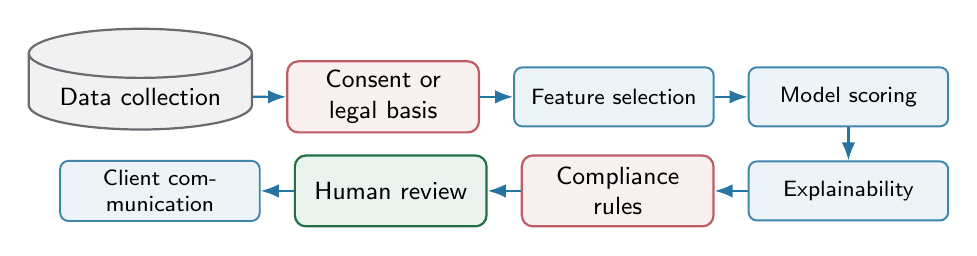
\begin{tikzpicture}[node distance=0.42cm]
		\node[data] (collect) {Data collection};
		\node[risk, right=of collect, text width=2.2cm] (basis) {Consent or legal basis};
		\node[smallflow, right=of basis] (features) {Feature selection};
		\node[smallflow, right=of features] (score) {Model scoring};
		\node[smallflow, below=of score] (xai) {Explainability};
		\node[risk, left=of xai, text width=2.2cm] (rules) {Compliance rules};
		\node[action, left=of rules, text width=2.2cm] (human) {Human review};
		\node[smallflow, left=of human] (comm) {Client communication};
		\draw[arrow] (collect) -- (basis);
		\draw[arrow] (basis) -- (features);
		\draw[arrow] (features) -- (score);
		\draw[arrow] (score) -- (xai);
		\draw[arrow] (xai) -- (rules);
		\draw[arrow] (rules) -- (human);
		\draw[arrow] (human) -- (comm);
	\end{tikzpicture}}
	\caption{Compliance-aware ML flow}
\end{figure}

\begin{figure}[H]
	\centering
	\begin{tabularx}{\textwidth}{L{0.23\textwidth} Y Y}
		\toprule
		\textbf{Risk} & \textbf{Example} & \textbf{Control}\\
		\midrule
		Privacy risk & Using data beyond client expectations. & Purpose limitation, consent/legal-basis checks, minimization.\\
		Bias risk & Model systematically excludes a protected or vulnerable group. & Bias testing, feature review, monitoring.\\
		Suitability risk & Product communication reaches unsuitable clients. & Suitability filters and human advisor review.\\
		Reputational risk & Client feels surveilled or pressured. & Transparent language and frequency caps.\\
		Operational risk & Wrong data extract sends wrong message. & QA, approvals, lineage, rollback plan.\\
		Model drift risk & Score quality decays after market changes. & Monitoring, recalibration, champion/challenger testing.\\
		\bottomrule
	\end{tabularx}
	\caption{Risk map for client marketing ML}
\end{figure}

\chapterimage{header_laptop_code.jpg}
\chapter{Day 7: Technical Bridge and Integrated Case Study}

\section{Module 13 - Technical Skill Bridge for the Internship}

\moduleblock
{Your computer engineering background transfers through SQL, Python, pandas, scikit-learn, APIs, data modeling, dashboards, workflow automation, documentation, and the ability to translate technical constraints to non-technical teams.}
{The highest-value intern contribution is usually not a complex model. It is a clear analysis, reliable data logic, a documented workflow, a useful prototype, or a dashboard that a business team can actually use.}
{SQL, pandas, scikit-learn, classification, clustering, feature engineering, model evaluation, dashboards, APIs, data cleaning, workflow automation, reporting, documentation.}
{\source{scikit-learn user guide}{https://scikit-learn.org/stable/user_guide}; \source{scikit-learn clustering guide}{https://scikit-learn.org/stable/modules/clustering.html}; \source{pandas groupby guide}{https://pandas.pydata.org/pandas-docs/stable/user_guide/groupby.html}; SQL customer analytics tutorials.}
{``SQL customer analytics tutorial''; ``Python customer segmentation scikit-learn tutorial''; ``bank churn prediction dataset tutorial''; ``propensity model Python scikit-learn''; ``marketing campaign analytics Python tutorial''.}
{Technical skill map; internship contribution map.}
{Which skills transfer directly? What should you learn before starting? What should you avoid overclaiming? What deliverables might be useful? How can you explain technical work to business teams?}
{Instead of promising an end-to-end AI system, propose a scoped analysis: define high-liquidity segment logic, validate data quality, build a simple propensity baseline, and produce a campaign measurement dashboard.}
{\term{Baseline model}{simple first model used for comparison}; \term{feature engineering}{creating useful variables}; \term{dashboard}{repeatable visual reporting layer}; \term{data dictionary}{definition of fields and business meaning}.}

\begin{figure}[H]
	\centering
	\resizebox{\textwidth}{!}{
	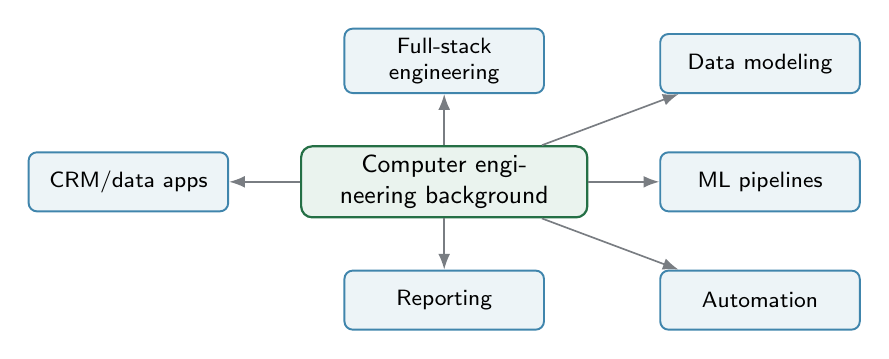
\begin{tikzpicture}[node distance=0.65cm and 0.9cm]
		\node[action, text width=3.4cm] (you) {Computer engineering background};
		\node[smallflow, above=of you] (fs) {Full-stack engineering};
		\node[smallflow, above right=of you] (dm) {Data modeling};
		\node[smallflow, right=of you] (ml) {ML pipelines};
		\node[smallflow, below right=of you] (auto) {Automation};
		\node[smallflow, below=of you] (report) {Reporting};
		\node[smallflow, left=of you] (crm) {CRM/data apps};
		\foreach \x in {fs,dm,ml,auto,report,crm}{\draw[softarrow] (you) -- (\x);}
	\end{tikzpicture}}
	\caption{Technical skill map}
\end{figure}

\begin{figure}[H]
	\centering
	\resizebox{\textwidth}{!}{
	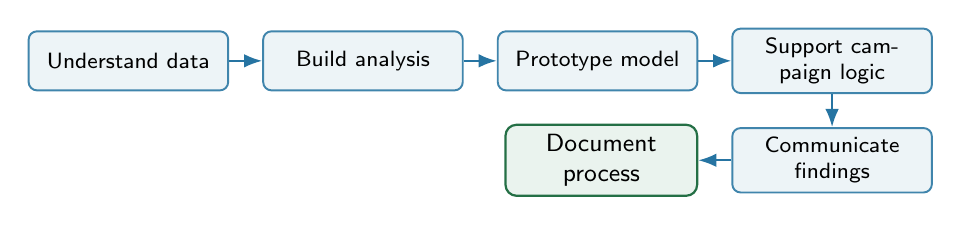
\begin{tikzpicture}[node distance=0.42cm]
		\node[smallflow] (understand) {Understand data};
		\node[smallflow, right=of understand] (analysis) {Build analysis};
		\node[smallflow, right=of analysis] (proto) {Prototype model};
		\node[smallflow, right=of proto] (logic) {Support campaign logic};
		\node[smallflow, below=of logic] (comm) {Communicate findings};
		\node[action, left=of comm, text width=2.2cm] (doc) {Document process};
		\draw[arrow] (understand) -- (analysis);
		\draw[arrow] (analysis) -- (proto);
		\draw[arrow] (proto) -- (logic);
		\draw[arrow] (logic) -- (comm);
		\draw[arrow] (comm) -- (doc);
	\end{tikzpicture}}
	\caption{Internship contribution map}
\end{figure}

\section{Module 14 - Integrated Mediolanum Case Study}

\moduleblock
{A fictional but realistic campaign: clients have high liquidity in current accounts but low investment product adoption. Marketing Clienti wants to support Family Bankers with educational content and compliant prompts for suitable planning conversations.}
{This case combines the whole guide: business model, CRM, segmentation, automation, ML scoring, compliance, advisor enablement, and measurement.}
{Business objective, data sources, segmentation, propensity model, consent and MiFID filters, journey execution, advisor alert, holdout group, measurement, risk interpretation.}
{Mediolanum public business model materials; CRM and marketing automation docs; GDPR and MiFID guidance; ML/uplift resources.}
{``high liquidity investment adoption banking campaign''; ``bank CRM propensity model investment meeting''; ``MiFID suitability investment advice marketing campaign''; ``banking customer segmentation high balance no investment''.}
{Full campaign architecture; data-to-action pipeline; client journey map; ML scoring workflow; measurement dashboard mockup.}
{What is the objective? What data is needed? Which filters are mandatory? What does the model predict? What does the Family Banker do? How is success measured?}
{The campaign should increase suitable investment conversations and improve client financial planning. ML is useful only when it creates a better, compliant, human-supported client interaction.}
{\term{High liquidity}{cash balance above a defined threshold}; \term{propensity to engage}{likelihood to respond or schedule a meeting}; \term{control group}{uncontacted comparison group}; \term{net inflows}{new assets entering managed or administered products}.}

\subsection{Case Walkthrough}

\begin{longtable}{L{0.24\textwidth} L{0.32\textwidth} L{0.34\textwidth}}
	\toprule
	\textbf{Step} & \textbf{Design choice} & \textbf{Reason}\\
	\midrule
	Business objective & Increase suitable investment conversations and improve client planning. & Links marketing activity to relationship value rather than simple product push.\\
	Data sources & Account balances, product holdings, risk profile, consent, campaign history, digital engagement, advisor relationship. & Combines need, eligibility, context, and contact permissions.\\
	Segmentation & High liquidity, no recent investment activity, active relationship, appropriate profile, no recent suppression. & Creates an audience that is business-relevant and operationally safe.\\
	ML model & Propensity to engage or schedule a meeting. & Ranks outreach priority without deciding product suitability.\\
	Compliance filters & Consent, MiFID suitability, communication preferences, exclusions, frequency caps. & Protects clients and the bank.\\
	Execution & App/email education, advisor alert, follow-up task. & Combines digital nudging with human relationship.\\
	Measurement & Open rate, meeting rate, conversion, net inflows, holdout comparison. & Separates attention from incremental business impact.\\
	Risks & Inappropriate targeting, privacy, over-contacting, weak explainability, advisor overload. & Shows what must be managed before scaling.\\
	\bottomrule
	\caption{Integrated high-liquidity case study design}
\end{longtable}

\begin{figure}[H]
	\centering
	\resizebox{\textwidth}{!}{
	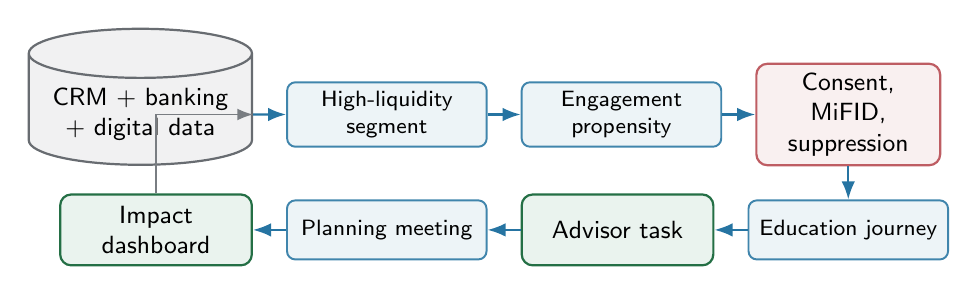
\begin{tikzpicture}[node distance=0.42cm]
		\node[data] (sources) {CRM + banking + digital data};
		\node[smallflow, right=of sources] (seg) {High-liquidity segment};
		\node[smallflow, right=of seg] (score) {Engagement propensity};
		\node[risk, right=of score, text width=2.1cm] (filters) {Consent, MiFID, suppression};
		\node[smallflow, below=of filters] (journey) {Education journey};
		\node[action, left=of journey, text width=2.2cm] (advisor) {Advisor task};
		\node[smallflow, left=of advisor] (meeting) {Planning meeting};
		\node[action, left=of meeting, text width=2.2cm] (measure) {Impact dashboard};
		\draw[arrow] (sources) -- (seg);
		\draw[arrow] (seg) -- (score);
		\draw[arrow] (score) -- (filters);
		\draw[arrow] (filters) -- (journey);
		\draw[arrow] (journey) -- (advisor);
		\draw[arrow] (advisor) -- (meeting);
		\draw[arrow] (meeting) -- (measure);
		\draw[softarrow] (measure) |- (sources);
	\end{tikzpicture}}
	\caption{Integrated Mediolanum case study flow}
\end{figure}

\begin{figure}[H]
	\centering
	\resizebox{\textwidth}{!}{
	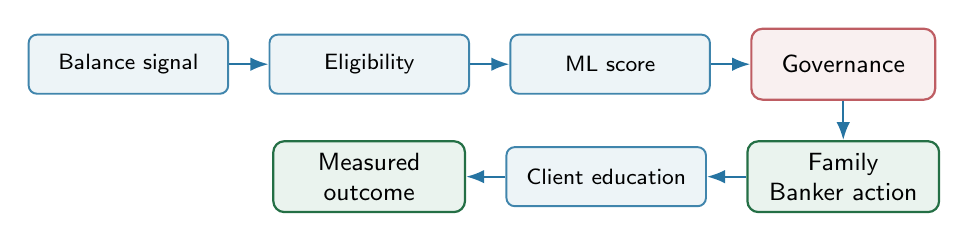
\begin{tikzpicture}[node distance=0.5cm]
		\node[smallflow] (bal) {Balance signal};
		\node[smallflow, right=of bal] (elig) {Eligibility};
		\node[smallflow, right=of elig] (score) {ML score};
		\node[risk, right=of score, text width=2.1cm] (govern) {Governance};
		\node[action, below=of govern, text width=2.2cm] (fb) {Family Banker action};
		\node[smallflow, left=of fb] (client) {Client education};
		\node[action, left=of client, text width=2.2cm] (outcome) {Measured outcome};
		\draw[arrow] (bal) -- (elig);
		\draw[arrow] (elig) -- (score);
		\draw[arrow] (score) -- (govern);
		\draw[arrow] (govern) -- (fb);
		\draw[arrow] (fb) -- (client);
		\draw[arrow] (client) -- (outcome);
	\end{tikzpicture}}
	\caption{Data-to-action pipeline for the case study}
\end{figure}

\begin{figure}[H]
	\centering
	\resizebox{\textwidth}{!}{
	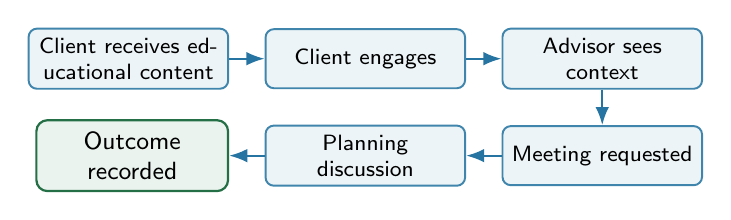
\begin{tikzpicture}[node distance=0.45cm]
		\node[smallflow] (notice) {Client receives educational content};
		\node[smallflow, right=of notice] (engage) {Client engages};
		\node[smallflow, right=of engage] (alert) {Advisor sees context};
		\node[smallflow, below=of alert] (meeting) {Meeting requested};
		\node[smallflow, left=of meeting] (plan) {Planning discussion};
		\node[action, left=of plan, text width=2.2cm] (record) {Outcome recorded};
		\draw[arrow] (notice) -- (engage);
		\draw[arrow] (engage) -- (alert);
		\draw[arrow] (alert) -- (meeting);
		\draw[arrow] (meeting) -- (plan);
		\draw[arrow] (plan) -- (record);
	\end{tikzpicture}}
	\caption{Client journey map for the case study}
\end{figure}

\begin{figure}[H]
	\centering
	\resizebox{\textwidth}{!}{
	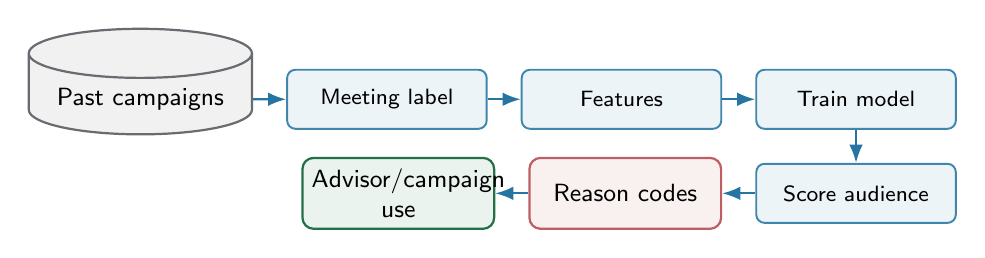
\begin{tikzpicture}[node distance=0.42cm]
		\node[data] (hist) {Past campaigns};
		\node[smallflow, right=of hist] (label) {Meeting label};
		\node[smallflow, right=of label] (feat) {Features};
		\node[smallflow, right=of feat] (model) {Train model};
		\node[smallflow, below=of model] (score) {Score audience};
		\node[risk, left=of score, text width=2.2cm] (explain) {Reason codes};
		\node[action, left=of explain, text width=2.2cm] (use) {Advisor/campaign use};
		\draw[arrow] (hist) -- (label);
		\draw[arrow] (label) -- (feat);
		\draw[arrow] (feat) -- (model);
		\draw[arrow] (model) -- (score);
		\draw[arrow] (score) -- (explain);
		\draw[arrow] (explain) -- (use);
	\end{tikzpicture}}
	\caption{ML scoring workflow for the case study}
\end{figure}

\begin{figure}[H]
	\centering
	\begin{tabularx}{\textwidth}{L{0.22\textwidth} C{0.16\textwidth} C{0.16\textwidth} C{0.16\textwidth} Y}
		\toprule
		\textbf{Metric} & \textbf{Target} & \textbf{Control} & \textbf{Lift} & \textbf{Interpretation}\\
		\midrule
		Open/app view rate & 54\% & 0\% & n/a & Exposure metric only.\\
		Meeting request rate & 8.4\% & 4.9\% & +3.5 pts & Stronger client engagement.\\
		Suitable conversation rate & 5.1\% & 3.2\% & +1.9 pts & Better advisor-supported planning.\\
		Investment conversion rate & 2.0\% & 1.4\% & +0.6 pts & Requires suitability and careful interpretation.\\
		Net inflows & higher & baseline & incremental & Needs time window and attribution rules.\\
		\bottomrule
	\end{tabularx}
	\caption{Measurement dashboard mockup for the case study}
\end{figure}

\chapterimage{header_library.jpg}
\chapter{Resources, Glossary, Interview Prep, and Cheat Sheet}

\section{Resource List With Links}

\begin{longtable}{L{0.25\textwidth} L{0.30\textwidth} L{0.35\textwidth}}
	\toprule
	\textbf{Area} & \textbf{Resource} & \textbf{Use}\\
	\midrule
	Mediolanum context & \source{Banca Mediolanum Investor Relations}{https://www.bancamediolanum.it/corporate/investors?lang=en} & Company profile, financial calendar, official investor materials.\\
	Mediolanum current results & \source{Q1 2026 press release}{https://www.bancamediolanum.it/static-assets/documenti/file/en/2026/05/07/CS_070526_ENG.pdf} & Current financial and operating metrics as of March 31, 2026.\\
	Mediolanum business model & \source{FY 2025 Results and Business Update}{https://www.emarketstorage.it/sites/default/files/comunicati/2026-02/20260203_177057.pdf} & Integrated business model, multi-channel model, group structure.\\
	Mediolanum annual report & \source{2024 Annual Financial Report}{https://www.bancamediolanum.it/static-assets/documenti/file/en/2025/06/26/Gruppo_Mediolanum_Bilancio_311224_ENG.pdf} & Strategy, business model, sustainability and governance context.\\
	Family Banker model & \source{Family Banker official site}{https://www.familybanker.it/} & Role of advisors and advisory proposition.\\
	Products & \source{Banca Mediolanum business areas}{https://www.bancamediolanum.it/aree-di-business} & Product families: banking, credit, investment, pension, protection.\\
	Banking basics & \source{ECB educational explainers}{https://www.ecb.europa.eu/ecb/educational/pricestab/html/index.en.html} & Simple official explanations on banking and monetary context.\\
	Banking basics & \source{Bank of Italy financial education}{https://www.bancaditalia.it/compiti/tutela-educazione/educazione-finanziaria/index.html?com.dotmarketing.htmlpage.language=1} & Italian consumer banking and financial education materials.\\
	CRM data model & \source{Salesforce Customer 360 Data Model}{https://help.salesforce.com/s/articleView?id=data.c360_a_c360datamodel.htm} & Customer 360 and data-model concepts.\\
	Financial services CRM & \source{Salesforce Financial Services Data Model}{https://developer.salesforce.com/docs/platform/data-models/guide/data-cloud-financial-services-overview.html} & Financial accounts, holdings, relationships, and data structures.\\
	Marketing automation & \source{Oracle Eloqua documentation}{https://docs.oracle.com/en/cloud/saas/marketing/eloqua.html} & Campaign planning and automation concepts.\\
	Data architecture & \source{Salesforce Data 360 architecture}{https://architect.salesforce.com/docs/architect/fundamentals/guide/data-360-architecture} & Data harmonization and activation patterns.\\
	Data governance & \source{BCBS 239}{https://www.bis.org/publ/bcbs239.htm} & Risk data aggregation and governance principles.\\
	ML in banking & \source{Retail banking churn framework}{https://link.springer.com/article/10.1186/s40854-023-00558-3} & Churn prediction concepts and class imbalance issues.\\
	CLV in banking & \source{Retail banking CLV paper}{https://arxiv.org/abs/2304.03038} & Product-based lifetime value modeling.\\
	Uplift modeling & \source{scikit-uplift user guide}{https://www.uplift-modeling.com/en/latest/user_guide/index.html} & Incremental response modeling for campaign targeting.\\
	Technical bridge & \source{scikit-learn user guide}{https://scikit-learn.org/stable/user_guide} & Classification, clustering, model evaluation.\\
	Technical bridge & \source{pandas groupby guide}{https://pandas.pydata.org/pandas-docs/stable/user_guide/groupby.html} & Customer analytics aggregation patterns.\\
	GDPR profiling & \source{EDPB profiling guidance}{https://www.edpb.europa.eu/our-work-tools/our-documents/guidelines/automated-decision-making-and-profiling_en} & Profiling and automated decision-making constraints.\\
	MiFID suitability & \source{ESMA suitability guidelines}{https://www.esma.europa.eu/document/guidelines-certain-aspects-mifid-ii-suitability-requirements-1} & Investment-advice suitability requirements.\\
	AI governance & \source{EBA Big Data and Advanced Analytics report}{https://eba.europa.eu/publications-and-media/press-releases/eba-report-identifies-key-challenges-roll-out-big-data-and} & Trust elements and governance pillars for analytics in banking.\\
	AI regulation & \source{European Commission AI Act overview}{https://commission.europa.eu/news/ai-act-enters-force-2024-08-01_en} & AI risk categories and governance expectations.\\
	\bottomrule
	\caption{Curated resource list}
\end{longtable}

\section{Header Image Credits}

\begin{table}[H]
	\centering
	\footnotesize
	\begin{tabularx}{\textwidth}{L{0.20\textwidth} L{0.45\textwidth} L{0.25\textwidth}}
		\toprule
		\textbf{Use} & \textbf{Image} & \textbf{License}\\
		\midrule
		Contents and schedule & \source{Study, study, study}{https://commons.wikimedia.org/wiki/File:Study,_study,_study_-_Flickr_-_pnoeric.jpg} & CC BY-SA 2.0\\
		Executive overview & \source{Banca Mediolanum sede}{https://commons.wikimedia.org/wiki/File:Banca_Mediolanum_sede.jpg} & CC BY-SA 4.0\\
		Banking and products & \source{Milan skyline, Porta Nuova business district}{https://commons.wikimedia.org/wiki/File:Milan_skyline_skyscrapers_of_Porta_Nuova_business_district.jpg} & CC0\\
		Organization and CRM & \source{Two people meeting with iPhone and iPad}{https://commons.wikimedia.org/wiki/File:Two_people_meeting_with_iphone_and_ipad_(Unsplash).jpg} & CC0\\
		Segmentation and automation & \source{Visitor Analytics Dashboard}{https://commons.wikimedia.org/wiki/File:Visitor_Analytics_Dashboard.jpg} & CC BY-SA 4.0\\
		ML and data pipelines & \source{Wikimedia Foundation Servers}{https://commons.wikimedia.org/wiki/File:Wikimedia_Foundation_Servers-8055_01.jpg} & CC BY-SA 3.0\\
		Compliance and governance & \source{European Parliament Strasbourg Hemicycle}{https://commons.wikimedia.org/wiki/File:European_Parliament_Strasbourg_Hemicycle_-_Diliff.jpg} & CC BY-SA 3.0\\
		Technical bridge and case study & \source{Pexels Luis Gomes coding laptop}{https://commons.wikimedia.org/wiki/File:Pexels-luis-gomes-546819.jpg} & CC0\\
		Resources & \source{Library bookshelf}{https://commons.wikimedia.org/wiki/File:Library_bookshelf.jpg} & CC0\\
		\bottomrule
	\end{tabularx}
\end{table}

\section{Interview and Internship Prep Questions}

\begin{multicols}{2}
\begin{enumerate}
	\item How would you explain Mediolanum's business model in two minutes?
	\item What makes the Family Banker model different from a branch-only bank?
	\item How can client marketing support an advisory network?
	\item What data would you need to identify high-liquidity clients?
	\item How would you distinguish a useful segment from a descriptive segment?
	\item What is a propensity model, and what should it not decide?
	\item Why is a holdout group important?
	\item What metrics would you use beyond click rate?
	\item How do consent and communication preferences affect campaign design?
	\item Why does MiFID suitability matter in investment-related campaigns?
	\item How would you explain model outputs to a non-technical stakeholder?
	\item What data quality checks would you run before launching a campaign?
	\item How would you document a campaign data extract?
	\item What is the difference between batch scoring and real-time scoring?
	\item How can ML help Family Bankers without replacing their judgment?
	\item What could go wrong with over-personalization?
	\item How would you evaluate whether a campaign improved business outcomes?
	\item What would you build in your first month as an intern?
\end{enumerate}
\end{multicols}

\section{Glossary}

\begin{multicols}{2}
\begin{description}[leftmargin=2.8cm, style=nextline, font=\sffamily\bfseries]
	\item[A/B test] Controlled experiment comparing variants.
	\item[AML] Anti-money laundering controls.
	\item[Asset gathering] Attracting and retaining client assets.
	\item[AUA/AUM] Assets under administration or management.
	\item[Bancassurance] Insurance distributed through a bank relationship.
	\item[Batch scoring] Scheduled model scoring for many clients.
	\item[CDP] Customer data platform.
	\item[Churn] Client inactivity, attrition, or relationship loss.
	\item[CLV] Predicted value of a client relationship over time.
	\item[Consent] Permission or legal basis for specific data use or communication.
	\item[Control group] Unexposed comparison group for measurement.
	\item[CRM] System and process for managing client relationships.
	\item[Cross-sell] Encouraging adoption of an additional relevant product.
	\item[Customer 360] Unified view of identity, products, behavior, interactions, and preferences.
	\item[ETL/ELT] Data movement and transformation patterns.
	\item[Family Banker] Mediolanum's advisory relationship role.
	\item[Feature] Model-ready variable derived from data.
	\item[Frequency cap] Limit on communication volume.
	\item[GDPR] EU personal-data protection regulation.
	\item[Holdout] Control group not exposed to a campaign.
	\item[Incrementality] Outcome caused by the intervention.
	\item[KYC] Know your customer checks.
	\item[Lead scoring] Ranking prospects or opportunities by expected value or readiness.
	\item[MiFID II] EU framework for investment services and investor protection.
	\item[Model drift] Decay or change in model behavior over time.
	\item[Net interest income] Interest earned on assets minus interest paid on funding.
	\item[Next best action] Ranked recommendation of the most appropriate next step.
	\item[Propensity] Probability of a behavior or response.
	\item[RFM] Recency, frequency, monetary value segmentation.
	\item[Suitability] Assessment that advice fits the client.
	\item[Suppression] Exclusion from a campaign due to rules.
	\item[Uplift] Incremental effect of a treatment.
	\item[XAI] Explainable AI methods and outputs.
\end{description}
\end{multicols}

\section{Final Cheat Sheet}

\begin{studybox}{The One-Sentence Answer}
Banca Mediolanum uses banking, investment, insurance, advisory, and digital services to manage long-term client relationships; Marketing Clienti uses CRM, segmentation, automation, and analytics to identify needs, support Family Bankers, personalize communication, and measure outcomes within strict privacy, compliance, explainability, and suitability constraints.
\end{studybox}

\begin{table}[H]
	\centering
	\begin{tabularx}{\textwidth}{L{0.22\textwidth} Y}
		\toprule
		\textbf{If asked about...} & \textbf{Say this}\\
		\midrule
		Mediolanum & A relationship-led, multi-channel bank and financial services group centered on Family Bankers and client needs.\\
		Bank revenue & Banks earn spread income, fees, commissions, and recurring asset-management/insurance economics while managing risk and capital.\\
		Client marketing & It coordinates lifecycle campaigns, education, engagement, retention, cross-sell, advisor enablement, and measurement.\\
		CRM & It operationalizes customer data: identity, products, interactions, campaigns, consents, preferences, and advisor relationships.\\
		Segmentation & It turns data into actionable audiences, but suitability and consent decide what can be done.\\
		Automation & It executes journeys, triggers, channels, suppressions, advisor tasks, and tracking.\\
		ML & It can score churn, propensity, uplift, CLV, channel preference, and next best action, but must be explainable and governed.\\
		Compliance & GDPR, MiFID suitability, consent, privacy, fairness, auditability, and human review shape every data-driven campaign.\\
		Internship contribution & Useful work is scoped, documented, measurable, and understandable to business teams.\\
		\bottomrule
	\end{tabularx}
	\caption{Final interview cheat sheet}
\end{table}

\section{Final Study Task}

Before the internship starts, write a two-page memo that proposes one campaign: the audience, data sources, compliance filters, message, advisor action, measurement plan, and one ML enhancement. Keep the model simple and the business logic explicit.

\end{document}
